\section{Experiments}
In this section, we first conduct experiments under both synthetic and real-world datasets. For each dataset, we investigate whether the methods fail to learn from samples within and outside HUA. Moreover, we perform additional experiments to demonstrate that even the Multivariate ERN, which employs distinct prior distributions, struggles to learn effectively within HUA. To compare performance, we use baselines including ERN~\cite{NEURIPS2020_aab08546} ($\mathcal{L}^{\mathrm{NLL}}+\lambda \mathcal{L}^{\mathrm{R}}$), and NLL-ERN ($\mathcal{L}^{\mathrm{NLL}}$). For experiments within HUA, we initialize the model within HUA by setting bias in the activation layer. %(See details in Appendix \ref{appendix_2}). 
Please refer to Appendix~\ref{appendix_2} for details about experimental setups and experiments about the sensitivity of hyperparameters.
%are shown in Appendix~\ref{appendix_2}.


\subsection{Performance on Cubic Regression Dataset}
To highlight the limitations of ERN, we compare its performance with our proposed \ours on cubic regression dataset~\cite{NEURIPS2020_aab08546} within HUA. Following~\cite{NEURIPS2020_aab08546}, we train models on $y=x^3+\epsilon$, where $\epsilon \sim \mathcal{N}(0,3)$. We conduct training over the interval $x \in[-4,4]$, and perform testing over $x \in \left[-6,-4) \cup (4,6\right]$.


\begin{figure}[t!]
\centering
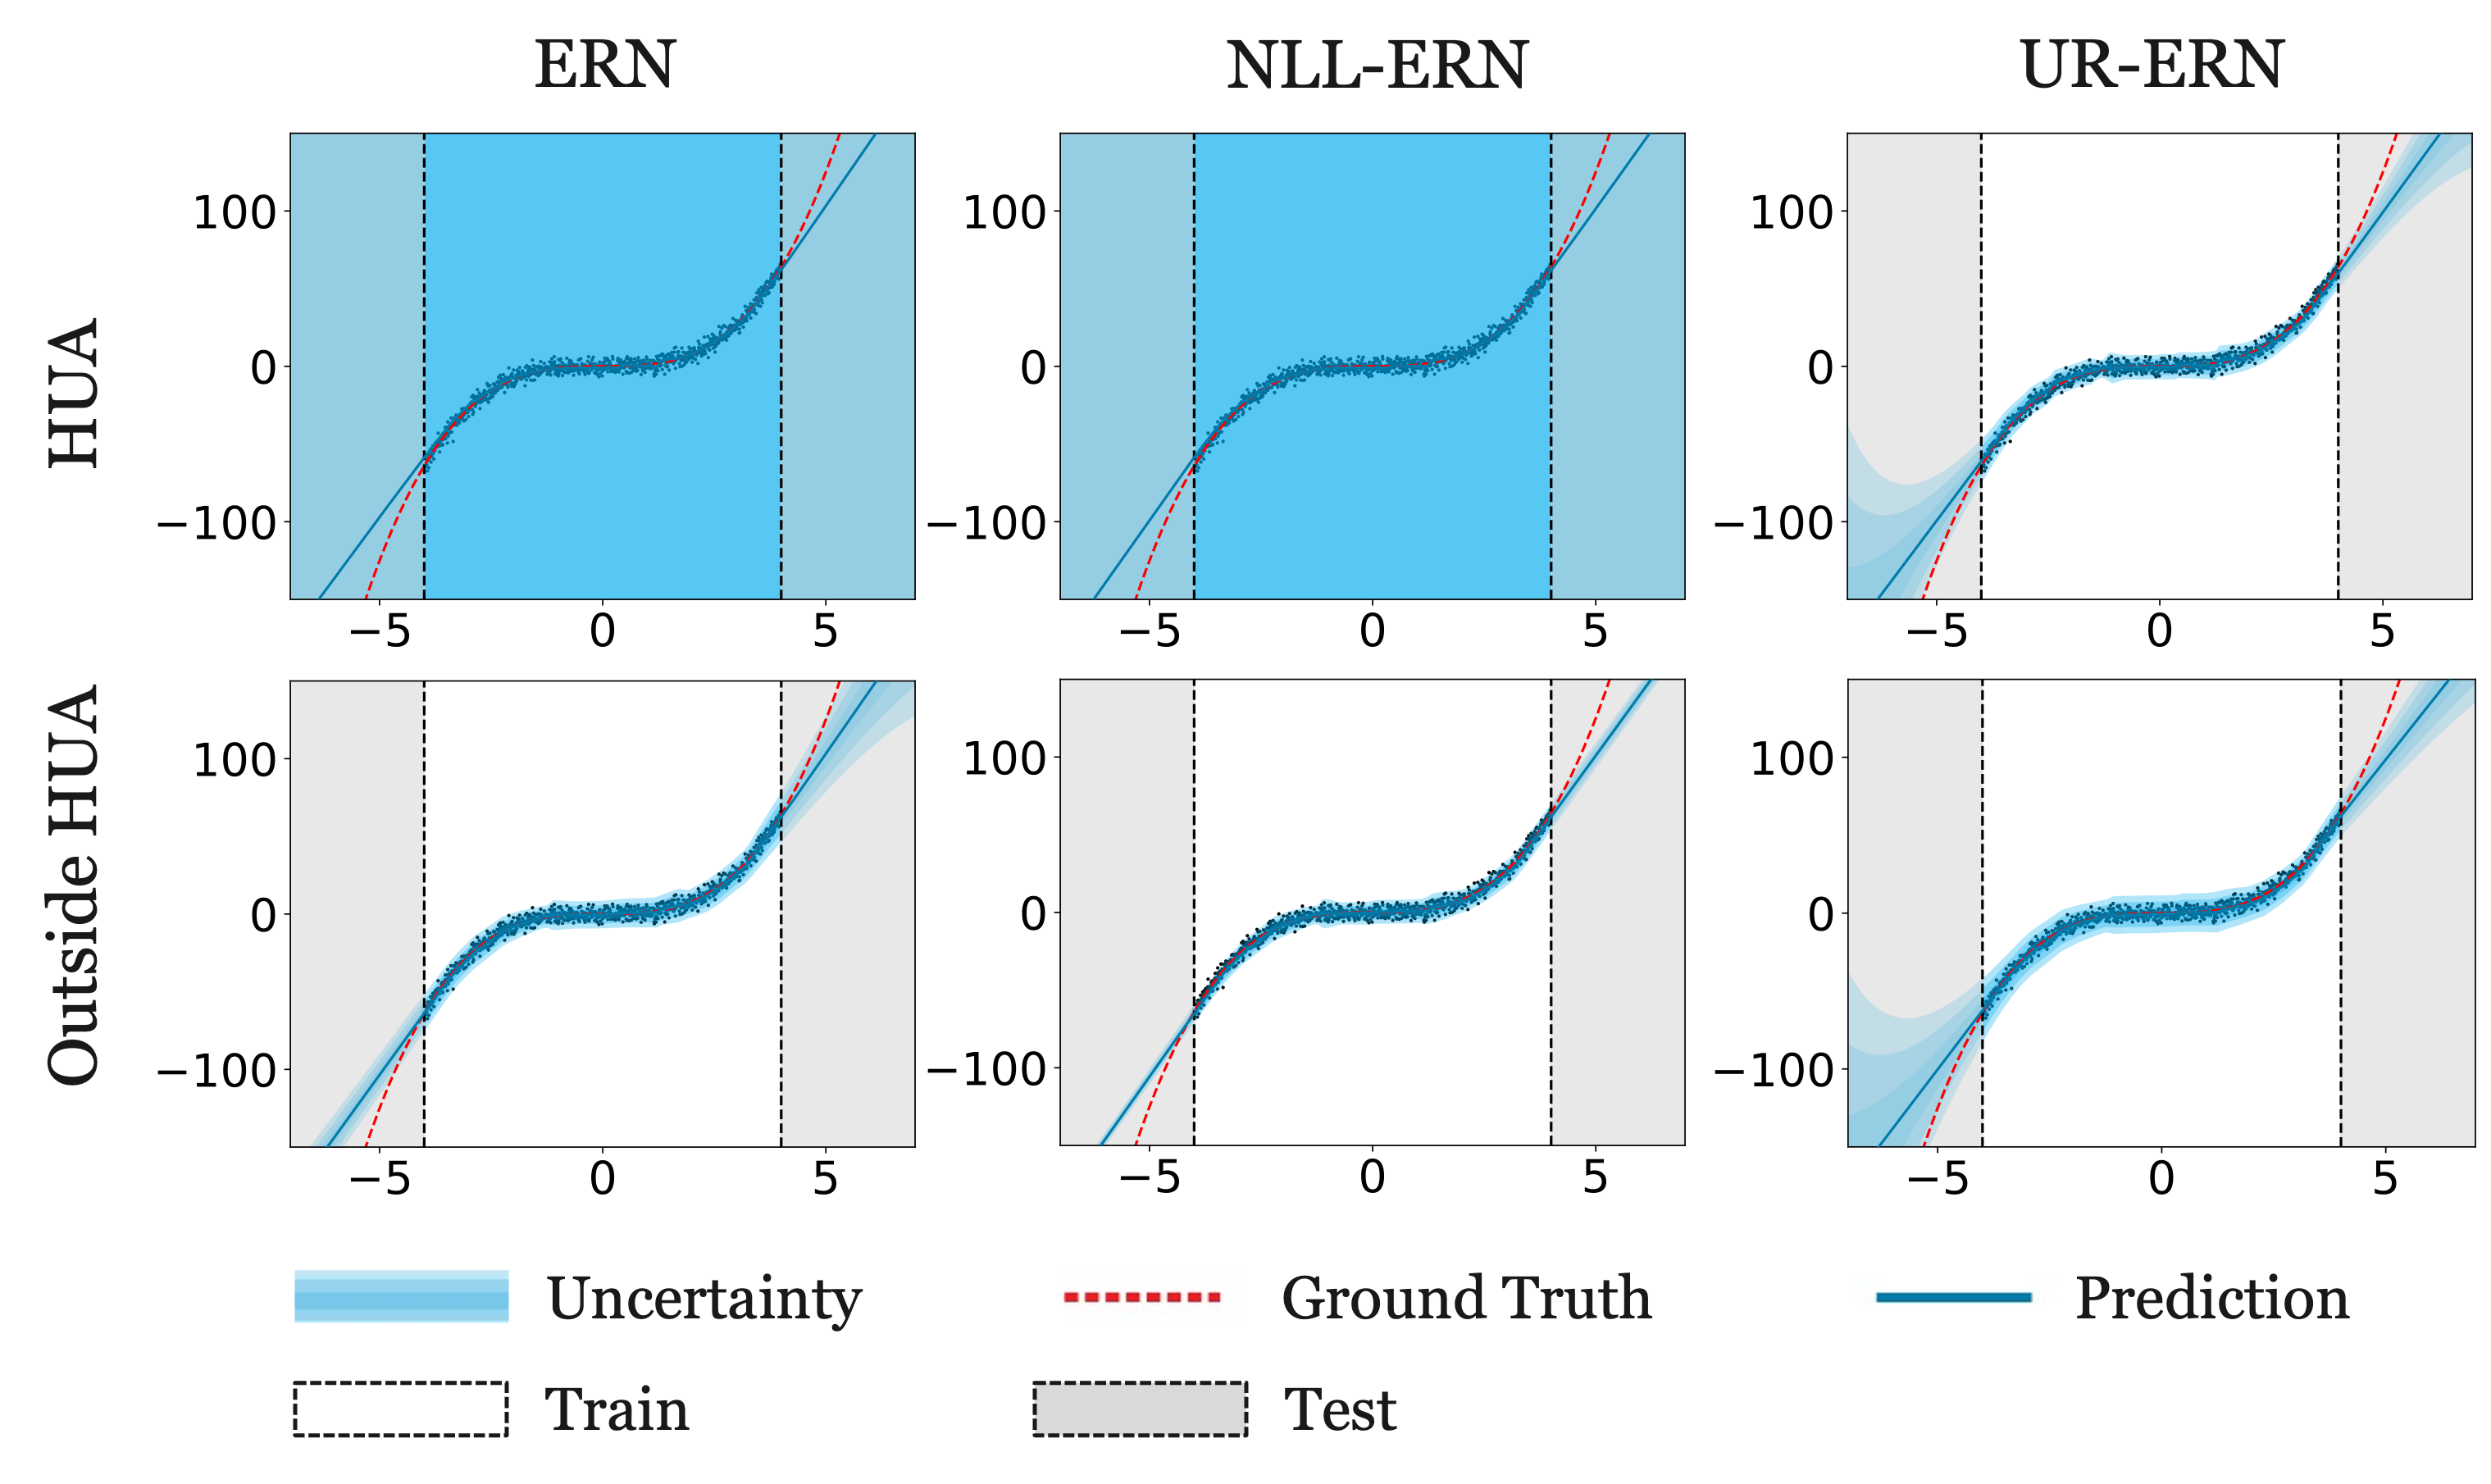
\includegraphics[width=0.9\columnwidth]{toy_dataset.png} % Reduce the figure size so that it is slightly narrower than the column. Don't use precise values for figure width.This setup will avoid overfull boxes.
\caption{Uncertainty estimation on Cubic Regression. The blue shade represents prediction uncertainty. An effective evidential model would cause the blue shade to cover the distance between the predicted value and the ground truth precisely. Up: Comparison of model performance within HUA. Down: Comparison of model performance outside HUA. \ours can cover the ground truth precisely under both within HUA and outside HUA.}
\label{fig:toy_dataset}
\end{figure}

% As demonstrated in Figure~\ref{fig:toy_dataset}, the blue shade represents uncertainty predicted by the models respectively. ERN struggles to update parameters within HUA, leading to high uncertainty prediction across the dataset, whereas \ours retains its training efficiency. This finding validates our previous theoretical analysis.
\subsubsection{Evaluation Metrics}
% Our proposed regularization mostly helps the model update $\alpha$ effectively within HUA, and the value of $\alpha$ is directly reflected in uncertainty prediction. Based on previous theoretical analysis, if the model fails to update $\alpha$ correctly, the uncertainty prediction will be unreasonably high.
% Therefore, we use uncertainty prediction as the evaluation metric. As is shown in~\ref{fig:toy_dataset}, it is represented as blue shade. For cubic regression, a better uncertainty prediction should be that the blue shade covers the the distance of predicted value and ground truth.
Our proposed regularization is mainly designed to help the model effectively update the parameter $\alpha$ within HUA. This is essential because, as our theoretical analysis has shown, if the model cannot properly update $\alpha$, the uncertainty prediction will become unreasonably high. Therefore, we have chosen uncertainty prediction as our evaluation metric. We visualize the experimental results of uncertainty estimation along with ground truth in Figure~\ref{fig:toy_dataset} and the uncertainty is represented by the blue shade. An accurate prediction in uncertainty would lead the blue shade to cover the distance between the predicted value and the ground truth precisely.

\subsubsection{Cubic Regression within HUA}
As illustrated in Figure~\ref{fig:toy_dataset}, where the blue shade represents the uncertainty predicted by the models, ERN encounters difficulties in updating parameters in the HUA, resulting in high uncertainty predictions across the dataset. In contrast, the proposed \ours maintains its training efficiency, effectively mitigating this issue. These observations validate our theoretical analysis, demonstrating the effectiveness of our proposed method. 
% We further explore the performance of these methods under normal settings (not within HUA). Figure~\ref{fig:toy_dataset_no_HUA} clearly shows the $\mathcal{L}^{\mathrm{R}}$ in $\mathcal{L}^{\mathrm{ERN}}$ helps the model get better uncertainty predictions, which our experiments validate the findings in~\citeauthor{NEURIPS2020_aab08546}. It can also be seen that the proposed \ours can perform well outside HUA, even better than ERN. This again demonstrates the effectiveness of our method.
\subsubsection{Cubic Regression outside HUA}
We extend our investigation to assess the performance of these methods under standard conditions (outside the HUA). Figure~\ref{fig:toy_dataset} illustrates that the inclusion of the term $\mathcal{L}^{\mathrm{R}}$ in $\mathcal{L}^{\mathrm{ERN}}$ contributes to more accurate uncertainty predictions, a result that aligns with the findings in~\citeauthor{NEURIPS2020_aab08546}. Moreover, the proposed \ours not only performs robustly in the HUA but also exhibits superior performance compared to the ERN outside the HUA. These observations further demonstrate the effectiveness of our method.



\begin{figure*}[t!]
  \centering
  \subfloat[Performance of model within HUA of Depth Estimation]{
    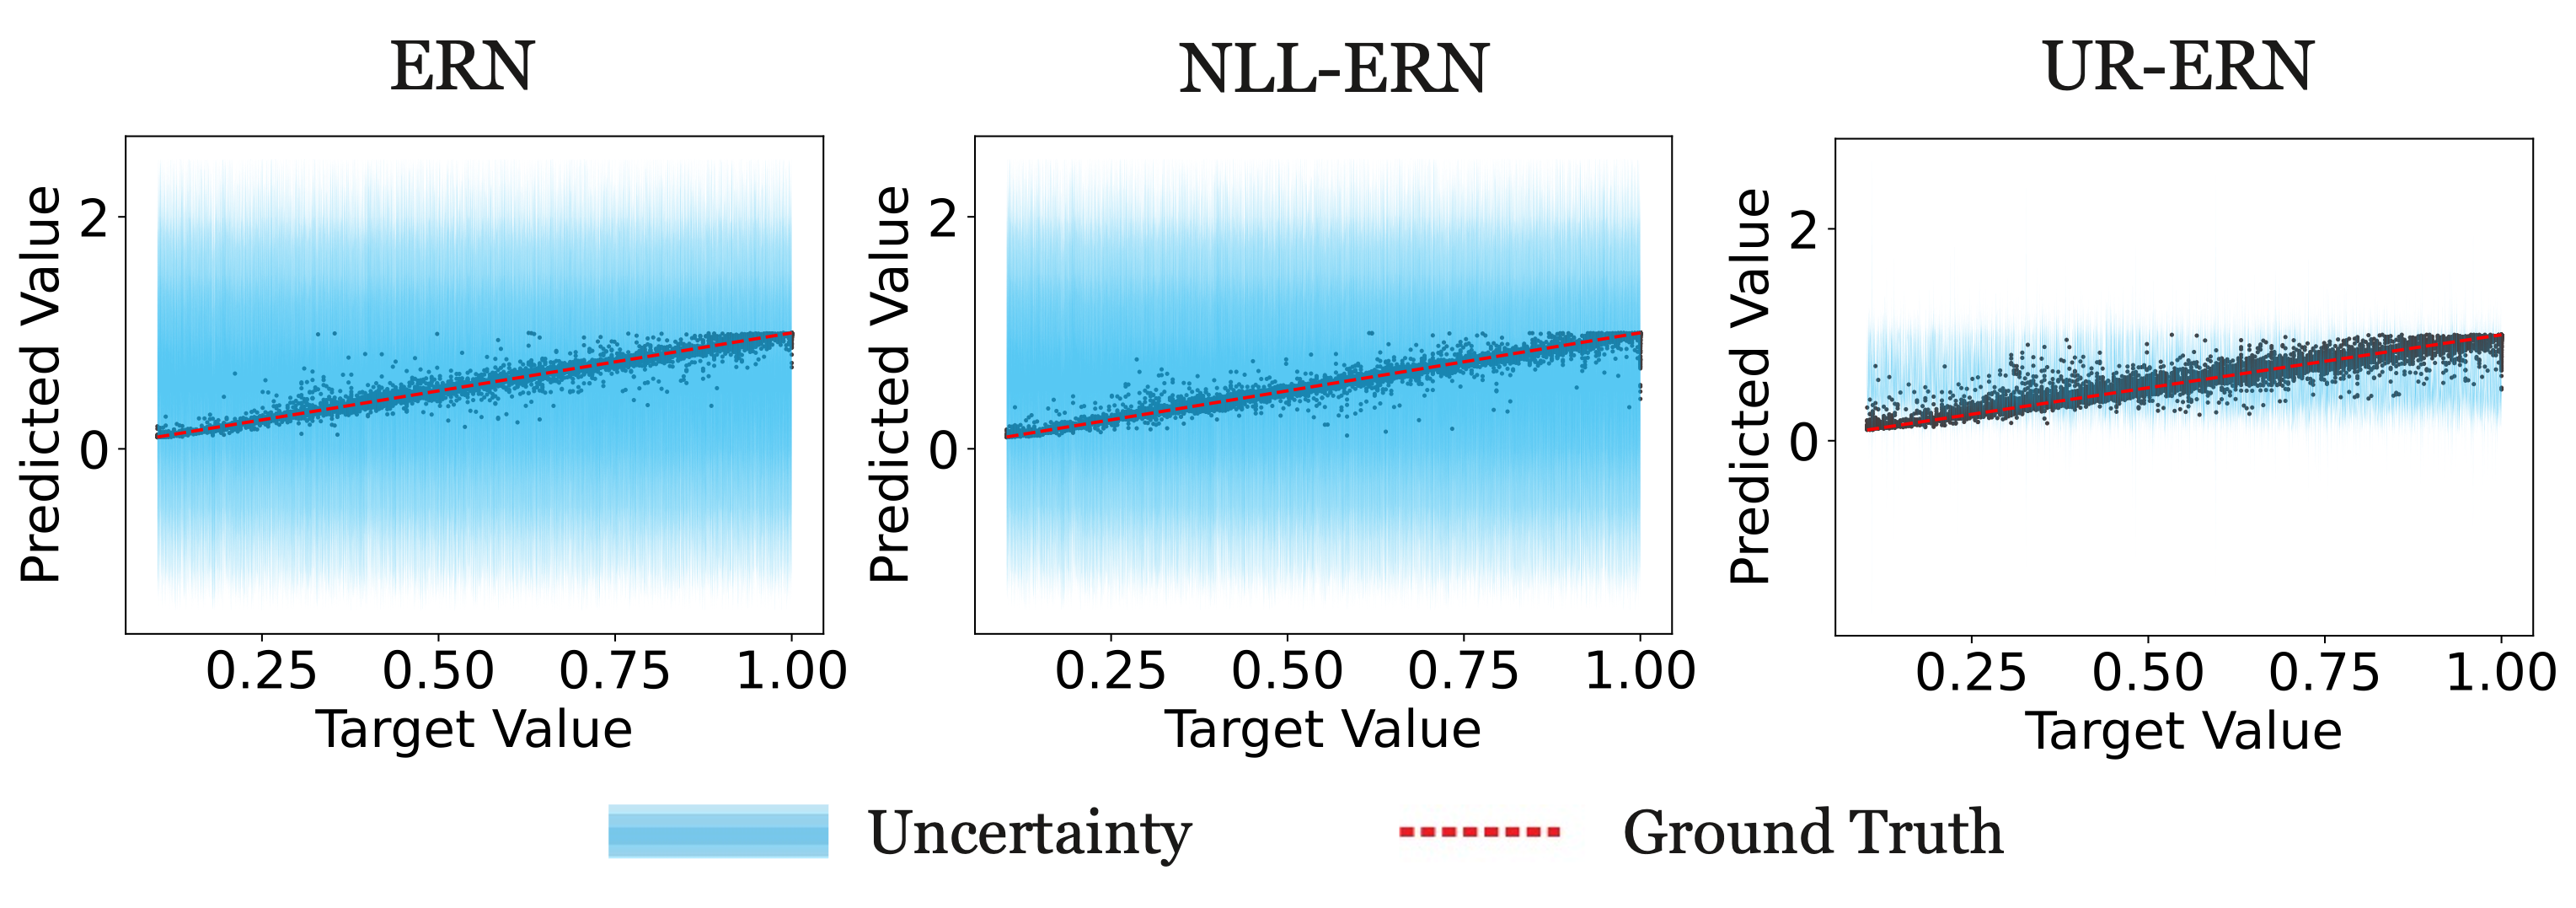
\includegraphics[width=0.5\linewidth]{depth_HUA_1.png}
  }
  \subfloat[RMSE with confidence]{
    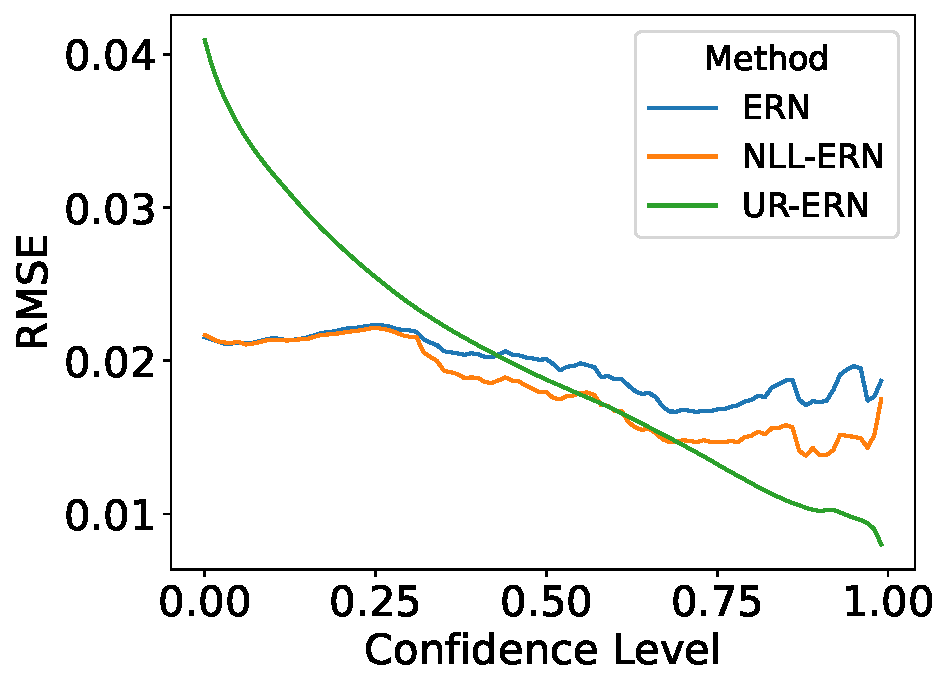
\includegraphics[width=0.22\linewidth]{depth_HUA_21.pdf}
  }
  \subfloat[Uncertainty calibration]{
    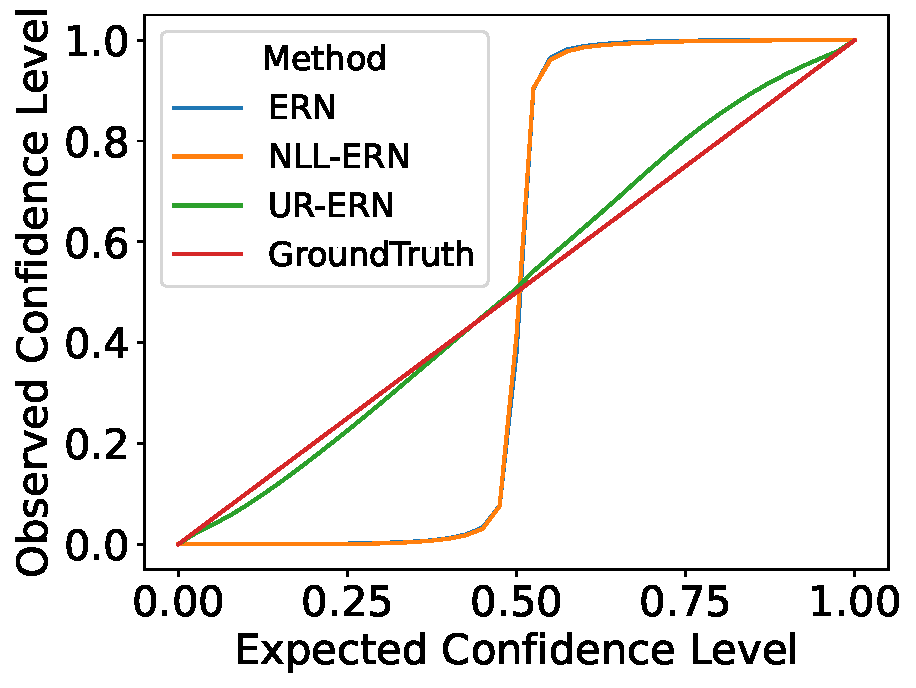
\includegraphics[width=0.22\linewidth]{depth_HUA_22.pdf}
  }
  \caption{Uncertainty prediction of Depth Estimation within HUA. (a) The blue shade represents prediction uncertainty. A good estimation of uncertainty should cover the gap between prediction and ground truth exactly. (b) Root Mean Square Error (RMSE) at various confidence levels. The evidential model with a larger confidence level should have a lower RMSE. (c) Uncertainty calibration calculated following~\citeauthor{kuleshov2018accurate}, the ideal curve is $y=x$. The calibration errors are 0.2261, 0.2250, and 0.0243 for ERN, NLL-ERN and UR-ERN, respectively.}
  \label{fig:depth_HUA}
\end{figure*}

\begin{figure*}[t!]
  \centering
  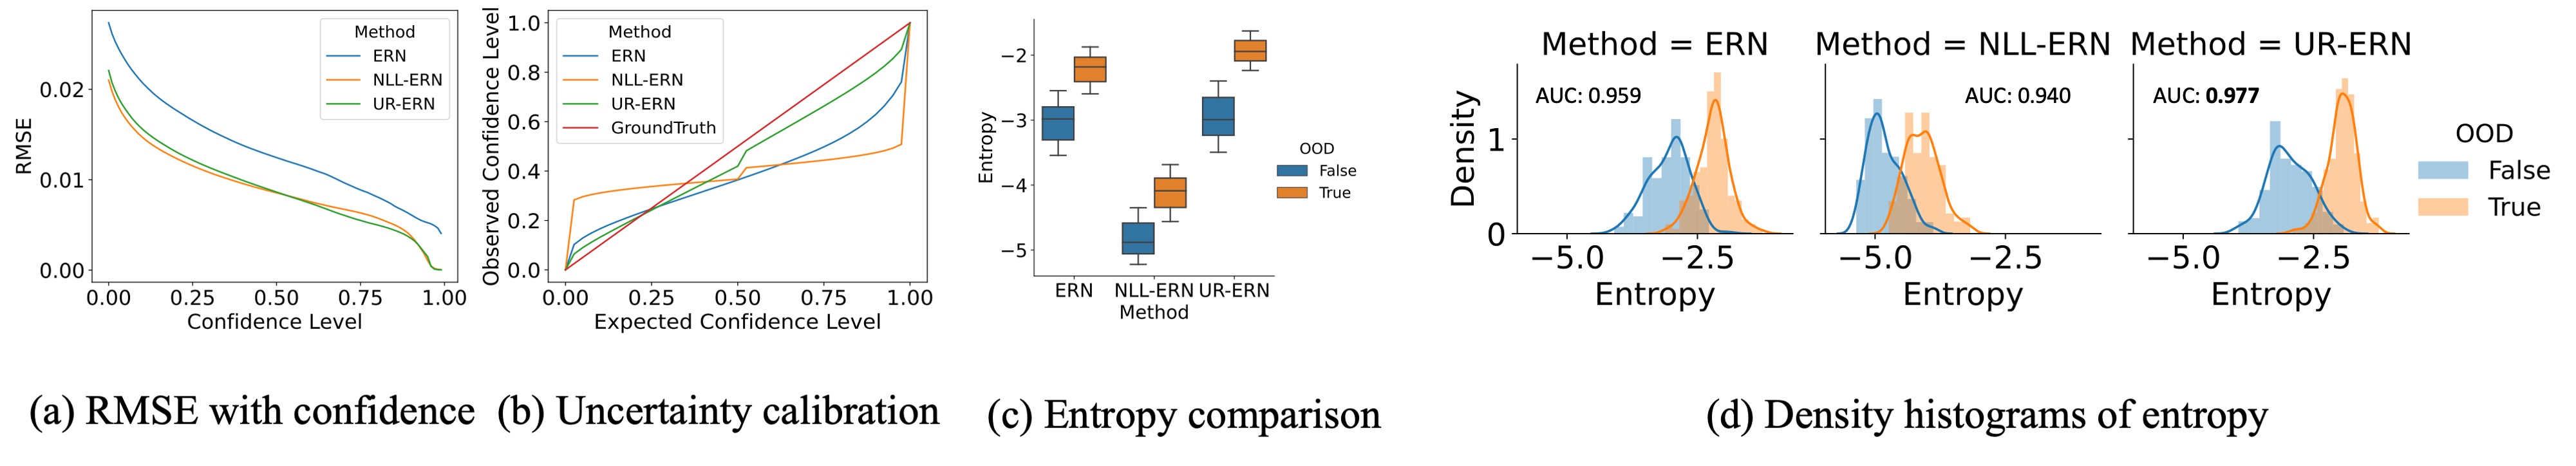
\includegraphics[width=0.95\linewidth]{depth_outside_HUA.jpg} 
  \caption{Uncertainty prediction of Depth Estimation outside HUA. (a) RMSE at various confidence levels. (b) Uncertainty calibration (ideal: $y=x$). The calibration errors are 0.1366, 0.1978, and 0.0289 for ERN, NLL-ERN and UR-ERN, respectively. (c) and (d) show OOD experimental results. (c) Entropy comparisons for different methods. (d) Density histograms of entropy. Entropy is calculated from $\sigma$, directly related to uncertainty. A good evidential model should be able to distinguish OOD data.}
  \label{fig:depth_outside_HUA}
\end{figure*}



\subsection{Performance on Monocular Depth Estimation}


We further evaluate the performance of our proposed \ours and ERN on more challenging real-world tasks. Monocular depth estimation is a task in computer vision aiming to predict the depth directly from an RGB image. We choose the NYU Depth v2 dataset~\cite{silberman2012indoor} for experiments.
For each pixel, there is a corresponding depth target. Following previous practice~\cite{NEURIPS2020_aab08546}, we train U-Net \cite{ronneberger2015u} style neural network as the backbone to learn evidential parameters. Similar to the previous section, we compare the performance of our \ours against ERN within HUA and outside HUA. Limited by space, additional experimental results are summarized in Appendix~\ref{appendix_2}.

\subsubsection{Evaluation Metrics}
For uncertainty in depth estimation, we first explore whether the models can correctly update parameters within HUA. Similarly, we choose the value of uncertainty as the evaluation metric. Similar to cubic regression, the blue shade in Figure~\ref{fig:depth_HUA}(a) depicts  predicted uncertainty. 
And the models that cannot learn from samples within HUA will exhibit excessively large blue shade areas, resulting from their high uncertainty prediction across the test set. 
%Models that cannot learn from samples within HUA will exhibit excessively large areas of blue shading, indicating high uncertainty predictions throughout the test set.

Following existing works~\citeauthor{NEURIPS2020_aab08546,kuleshov2018accurate}, we also use cutoff curves and calibration curves to compare the performance of uncertainty estimation. Inspired by previous work~\cite{NEURIPS2020_aab08546}, we further test how the models perform when faced with OOD data. An effective evidential model should predict high uncertainty for OOD data and can distinguish the OOD data. The OOD experimental setup is the same as~\citeauthor{NEURIPS2020_aab08546} for comparison.

% \begin{figure*}
%   \centering
%   \begin{tabular}{ccc}
%   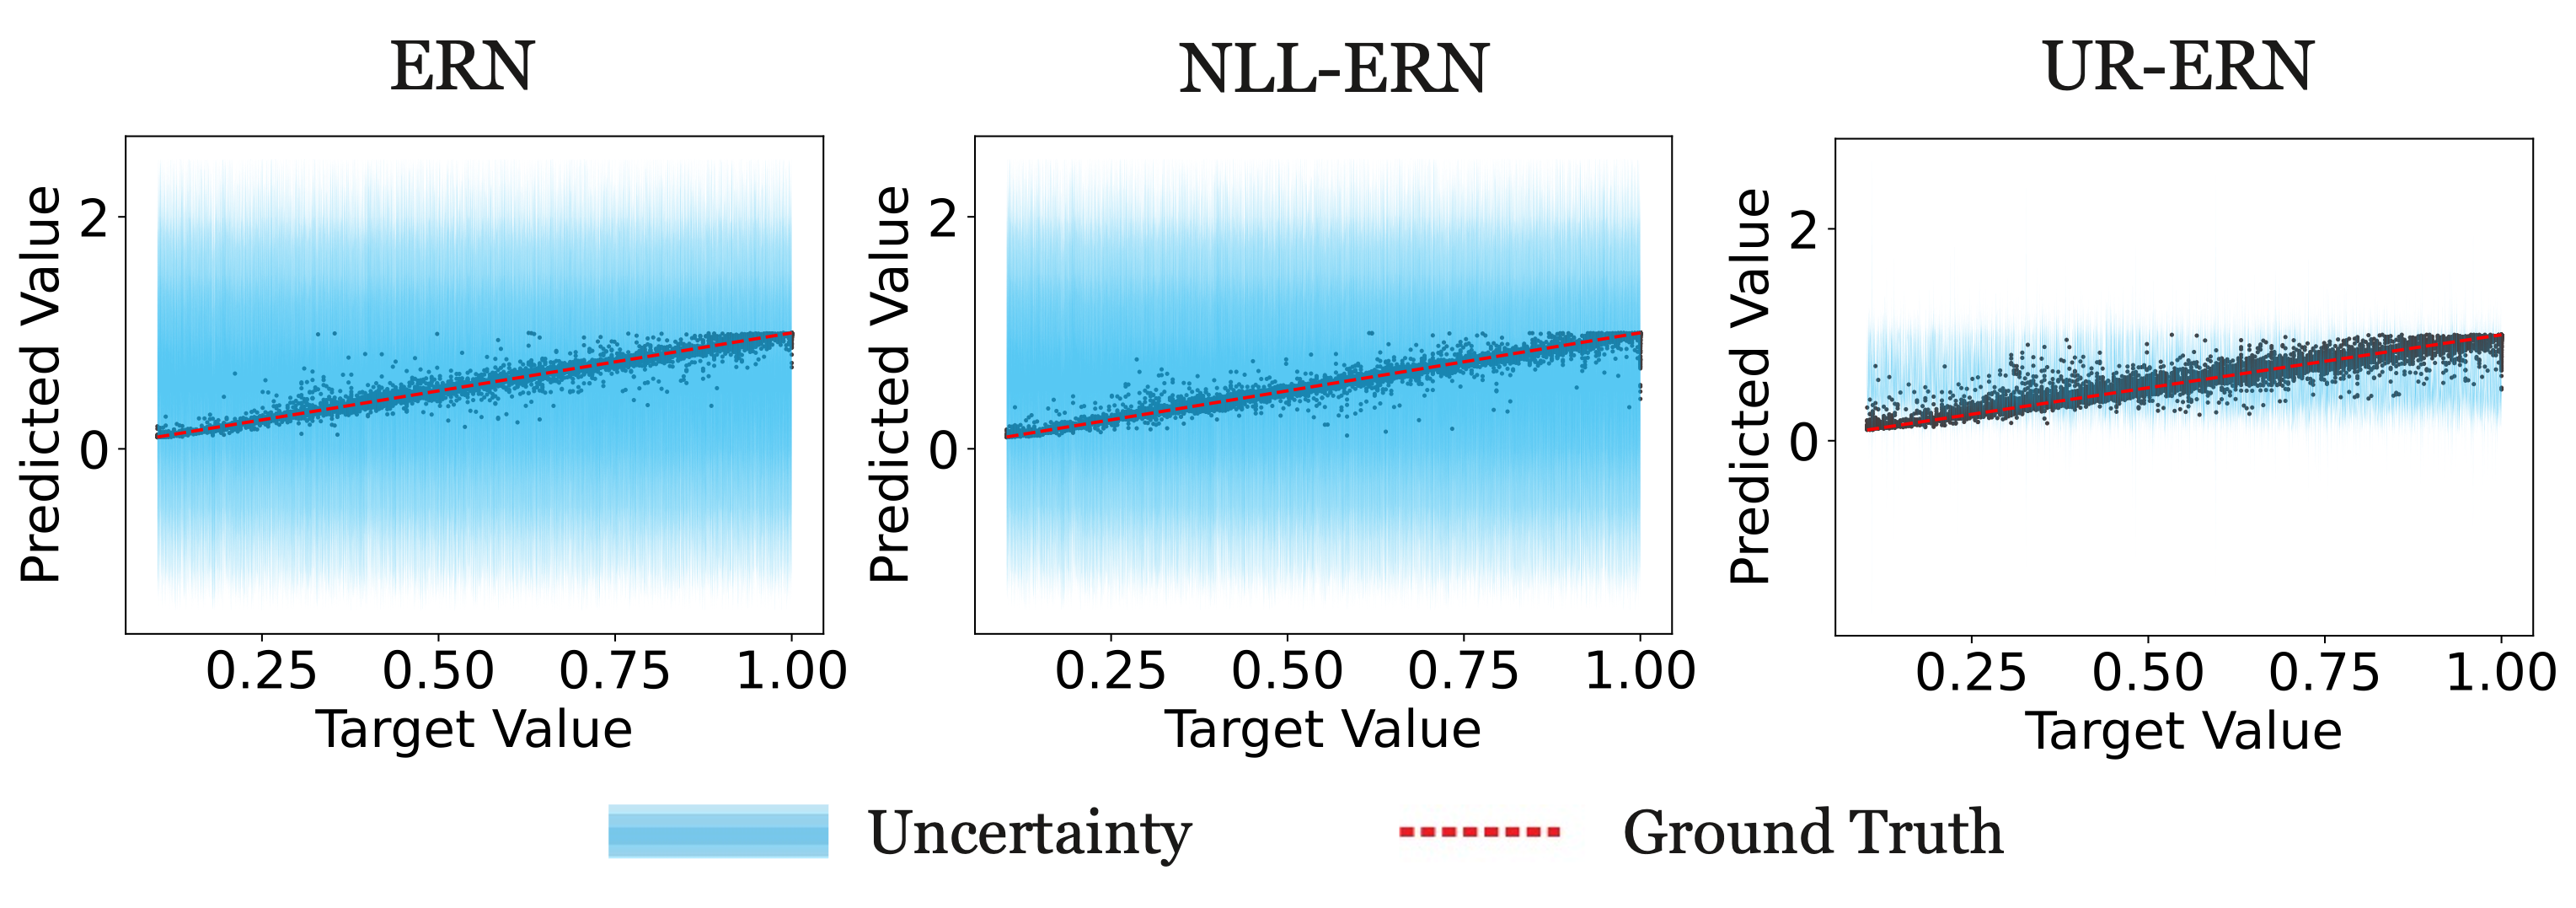
\includegraphics[width=0.5\linewidth]{depth_HUA_1.png} & 
% 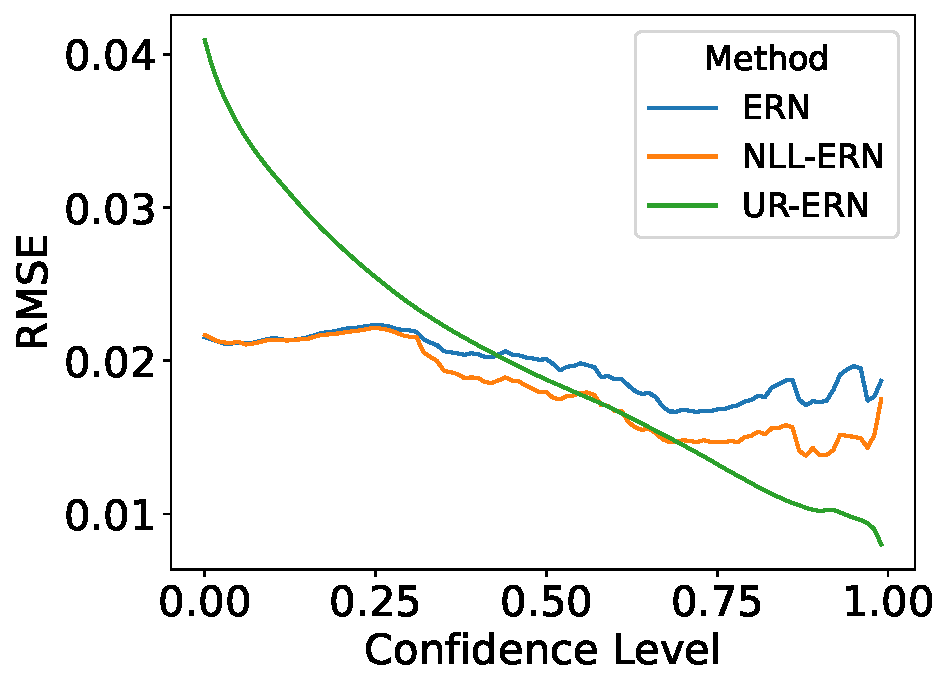
\includegraphics[width=0.22\linewidth]{depth_HUA_21.pdf}    & 
% 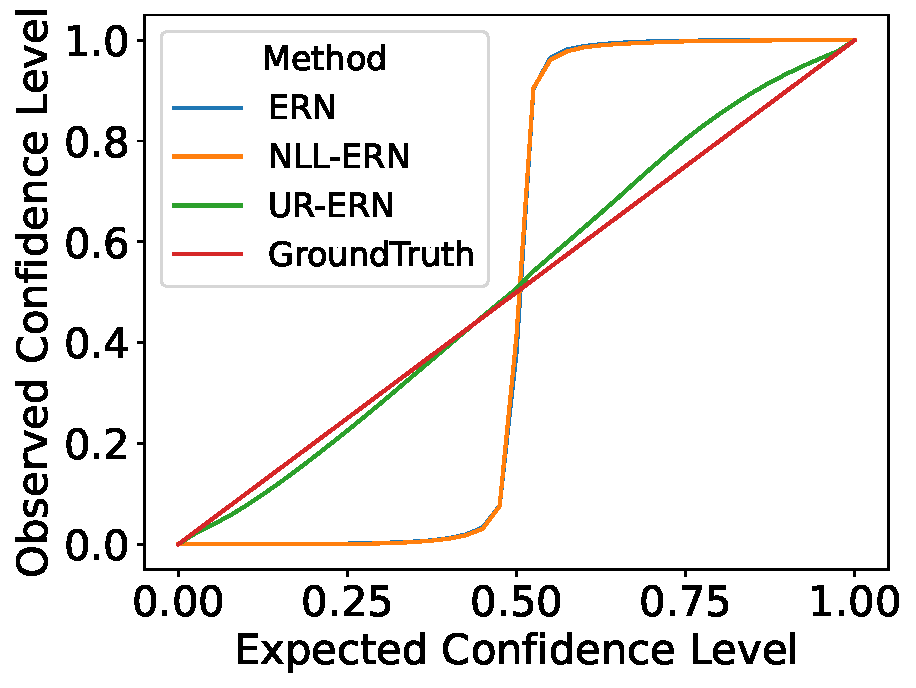
\includegraphics[width=0.22\linewidth]{depth_HUA_22.pdf} \\
% (a) Performance of model within HUA of Depth Estimation & (b) \hua{RMSE at} & (c)
%   \end{tabular}
%   \caption{Uncertainty prediction of Depth Estimation within HUA. (a) The blue shade represents prediction uncertainty. A good estimation of uncertainty should cover the gap between prediction and ground truth exactly. (b) Root Mean Square Error (RMSE) at various confidence levels. The evidential model with a larger confidence level should have a lower RMSE. (c) Uncertainty calibration calculated following~\citeauthor{kuleshov2018accurate}, the ideal curve is $y=x$.}
%   \label{fig:depth_HUA}
%   % \label{fig:depth_HUA1}
% \end{figure*}


% \begin{figure*}[h!]
%   \centering
%   \begin{tabular}{cccc}
%      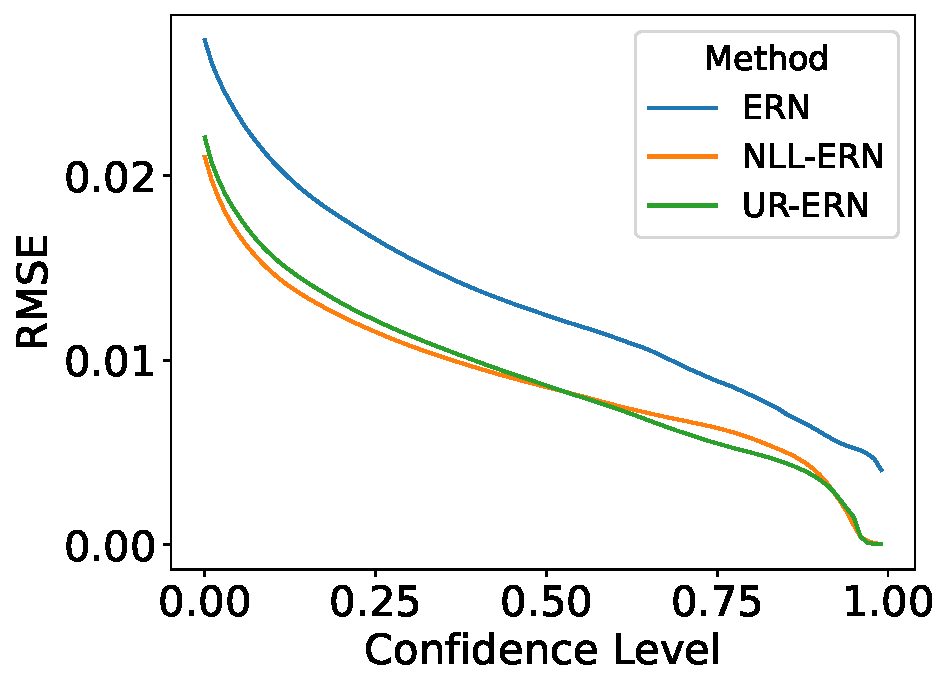
\includegraphics[width=0.15\linewidth]{depth_outside_HUA_1.pdf}  &
%      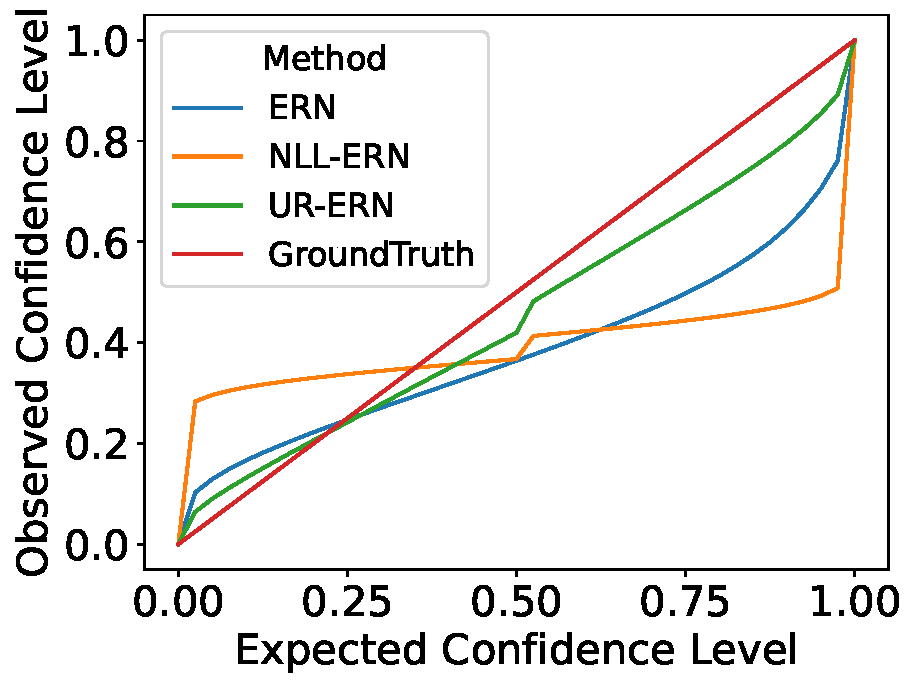
\includegraphics[width=0.15\linewidth]{depth_outside_HUA_2.pdf} &  
%      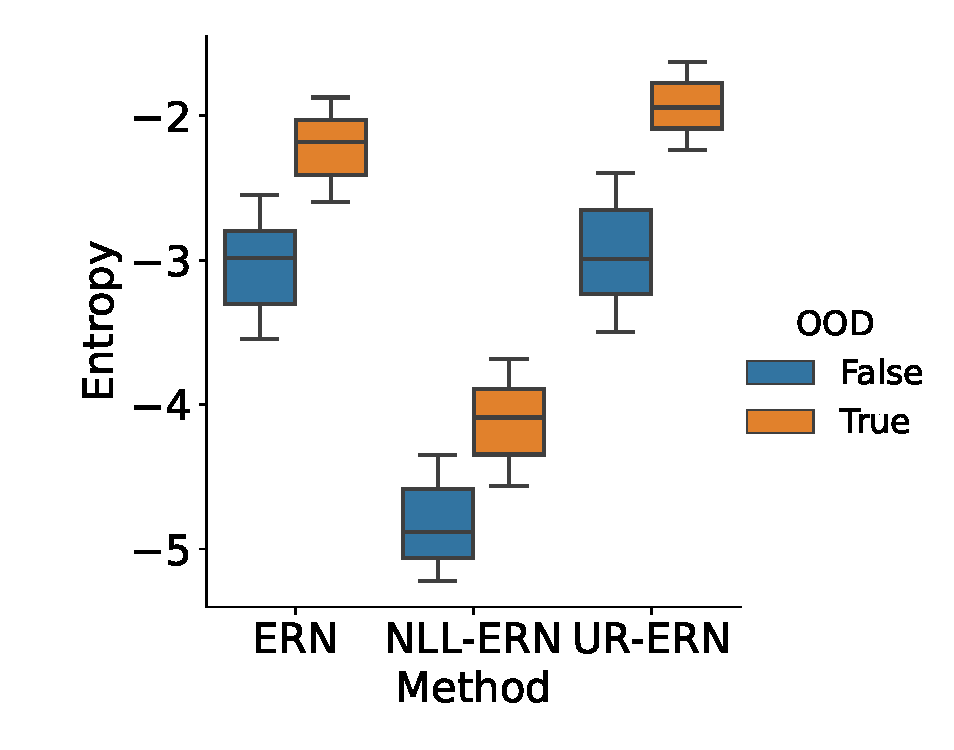
\includegraphics[width=0.2\linewidth]{depth_outside_HUA_3.pdf}  &
%      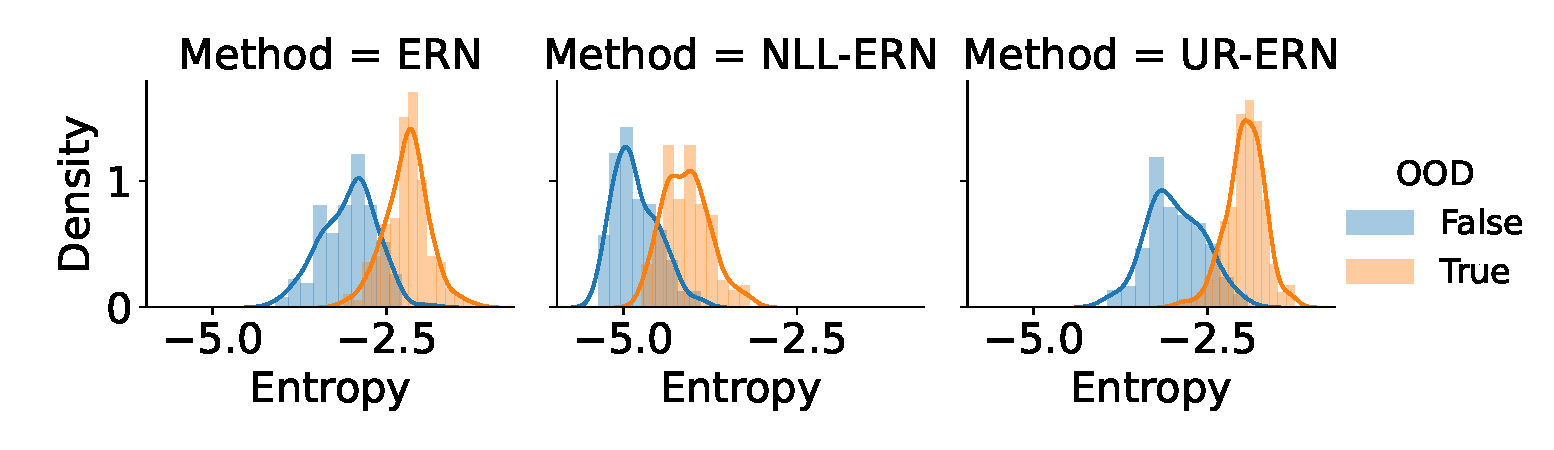
\includegraphics[width=0.45\linewidth]{depth_outside_HUA_4.pdf} \\
%       (a) & (b)  & (c)  & (d) 
%   \end{tabular}
%   \caption{\hua{maybe align with PPT and add as one picture }Uncertainty prediction of depth estimation outside HUA. (a) RMSE at various confidence levels. (b) Uncertainty calibration (ideal: $y=x$). (c) and (d) show OOD experimental results. (c) Entropy comparisons for different methods. (d) Density histograms of entropy. Entropy is calculated from $\sigma$, directly related to uncertainty. A good evidential model should be able to distinguish OOD data.}
%   \label{fig:depth_outside_HUA}
% \end{figure*}

% \begin{figure*}[h!]
%   \centering
%   \subfloat[]{
%     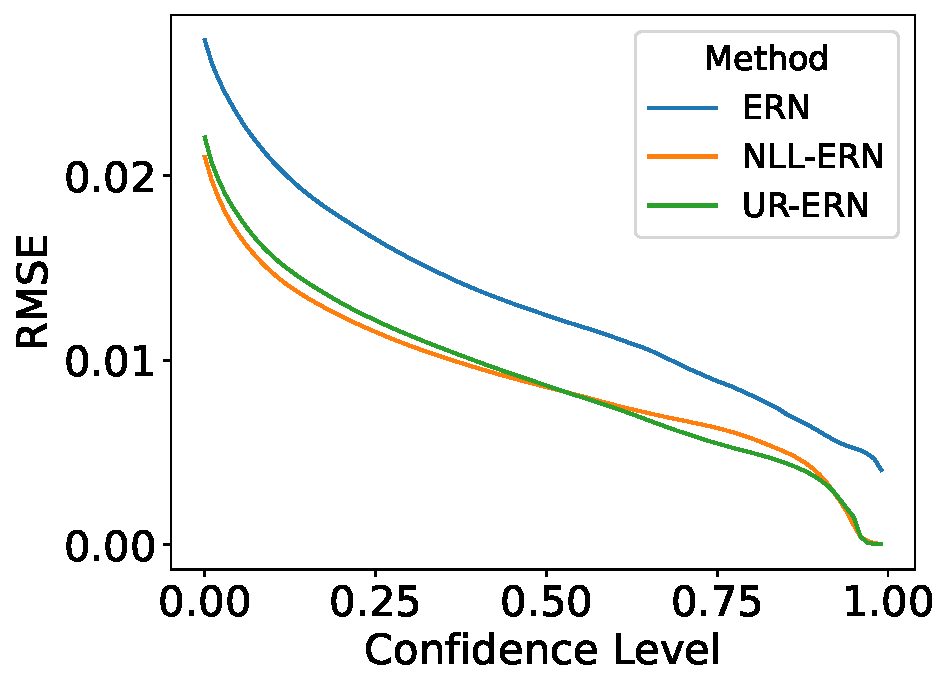
\includegraphics[width=0.155\linewidth]{depth_outside_HUA_1.pdf}
%   }
%   \subfloat[]{
%     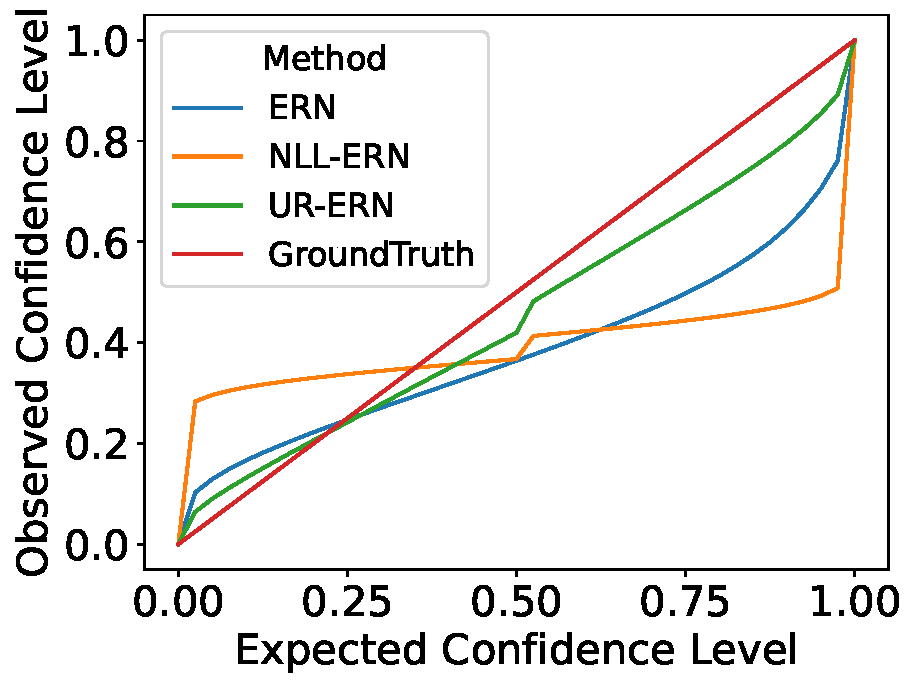
\includegraphics[width=0.15\linewidth]{depth_outside_HUA_2.pdf}
%   }
%   \subfloat[Entropy comparison]{
%     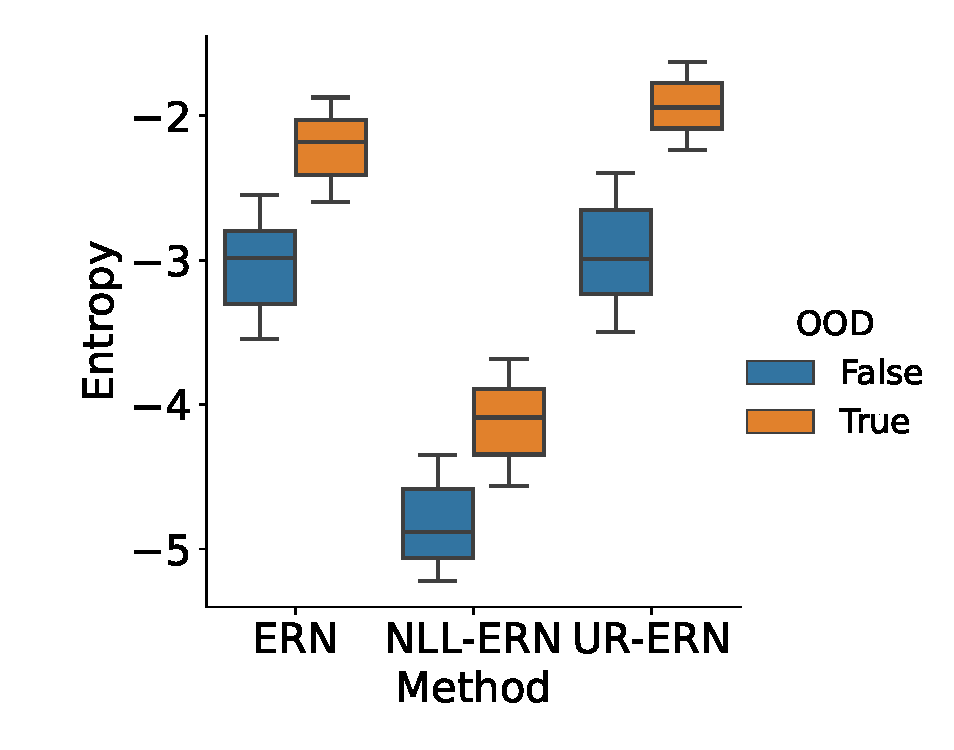
\includegraphics[width=0.2\linewidth]{depth_outside_HUA_3.pdf}
%   }
%   \subfloat[Density histograms of entropy]{
%     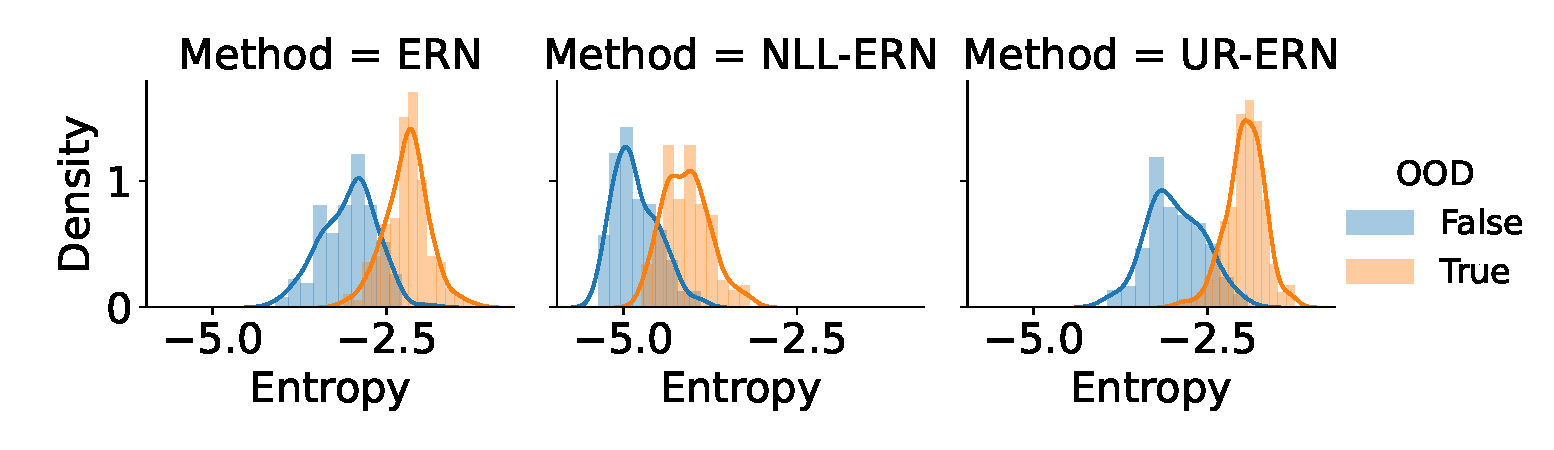
\includegraphics[width=0.45\linewidth]{depth_outside_HUA_4.pdf}
%   }
%   \caption{Uncertainty prediction of depth estimation outside HUA. (a) RMSE at various confidence levels. (b) Uncertainty calibration (ideal: $y=x$). (c) and (d) show OOD experimental results. (c) Entropy comparisons for different methods. (d) Density histograms of entropy. Entropy is calculated from $\sigma$, directly related to uncertainty. A good evidential model should be able to distinguish OOD data.}
%   \label{fig:depth_outside_HUA}
% \end{figure*}



\subsubsection{Monocular Depth Estimation within HUA}
As illustrated in Figure~\ref{fig:depth_HUA}, ERN with $\mathcal{L}^{\mathrm{R}}$ or not, struggles to update parameters effectively within the HUA, leading to suboptimal uncertainty estimation. This constraint forms a significant impediment to effective learning from particular samples. In contrast, the proposed \ours successfully navigates this challenge, demonstrating the capacity to learn from these specific samples and to efficiently estimate uncertainty, mirroring the behavior observed in normal regions.

% \begin{figure}
%   \centering
%   \subfloat[]{
%     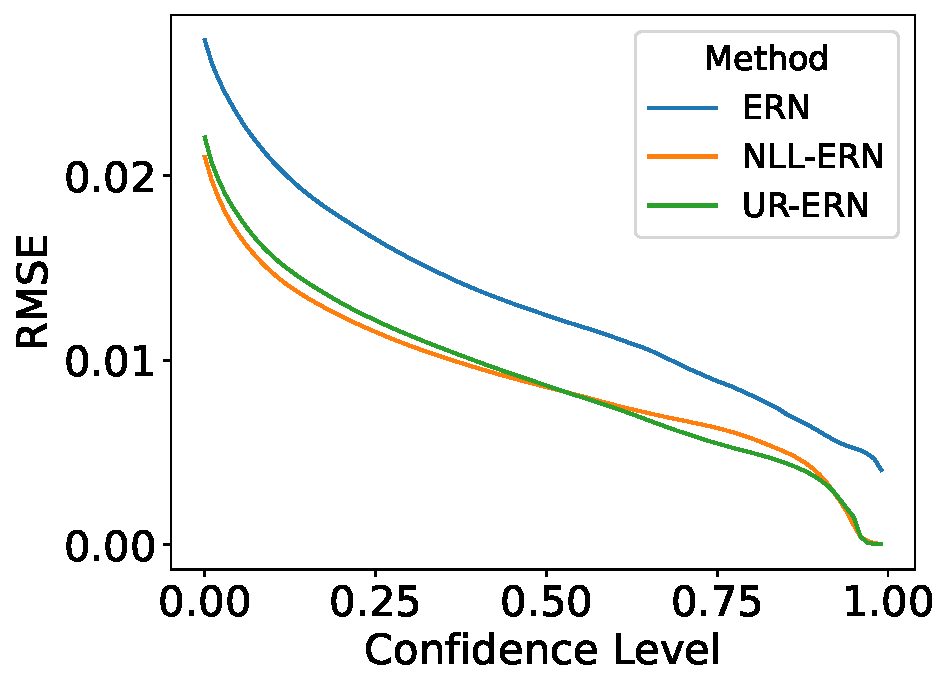
\includegraphics[width=0.45\linewidth]{depth_outside_HUA_1.pdf}
%   }
%   \subfloat[]{
%     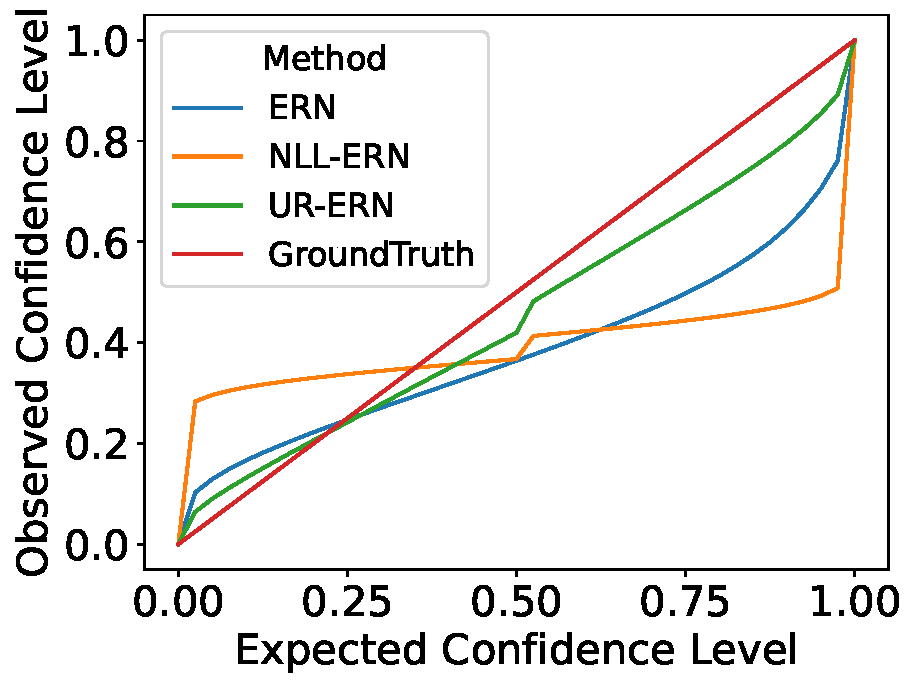
\includegraphics[width=0.45\linewidth]{depth_outside_HUA_2.pdf}
%   }\\
%   \subfloat[]{
%     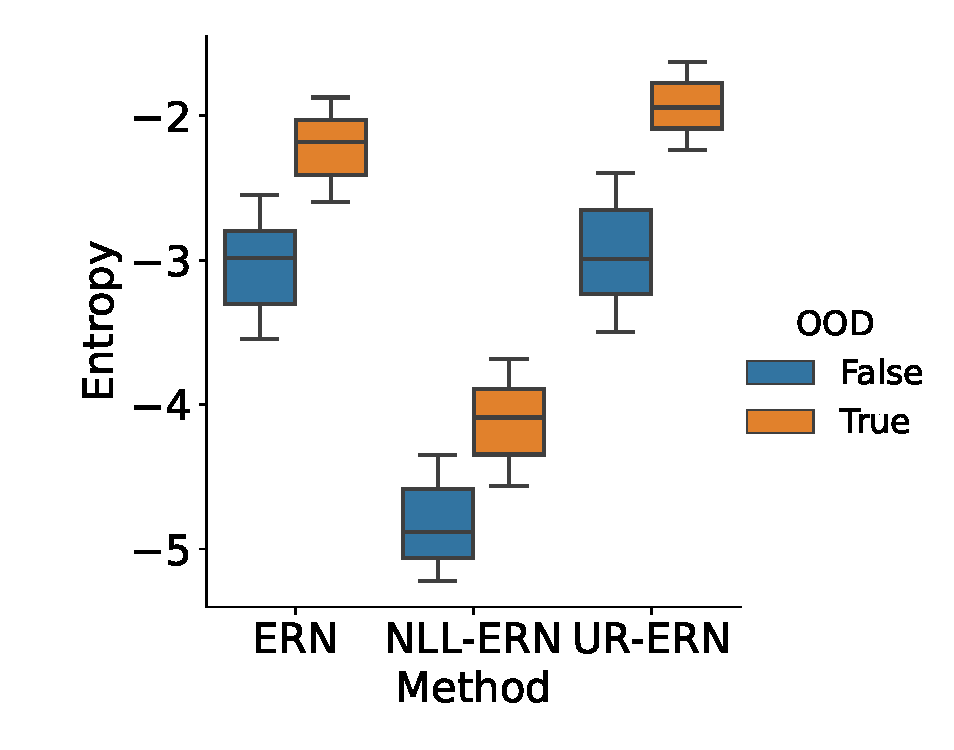
\includegraphics[width=0.5\linewidth]{depth_outside_HUA_3.pdf}
%   }\\
%   \subfloat[]{
%     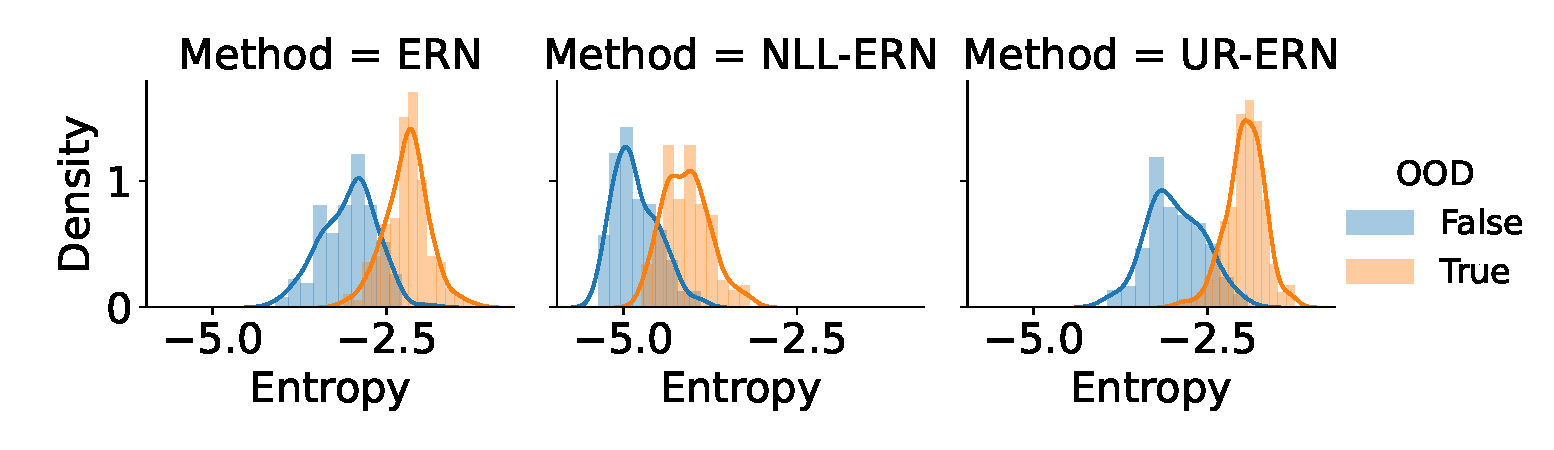
\includegraphics[width=0.9\linewidth]{depth_outside_HUA_4.pdf}
%   }
%   \caption{Uncertainty prediction of depth estimation outside HUA. (a) RMSE at various confidence levels. (b) Uncertainty calibration (ideal: $y=x$). (c) and (d) show OOD experimental results. (c) Entropy comparisons for different methods. (d) Density histograms of entropy. Entropy is calculated from $\sigma$, directly related to uncertainty. A good evidential model should be able to distinguish OOD data.}
%   \label{fig:depth_outside_HUA}
% \end{figure}


% \begin{figure}
% \centering
% 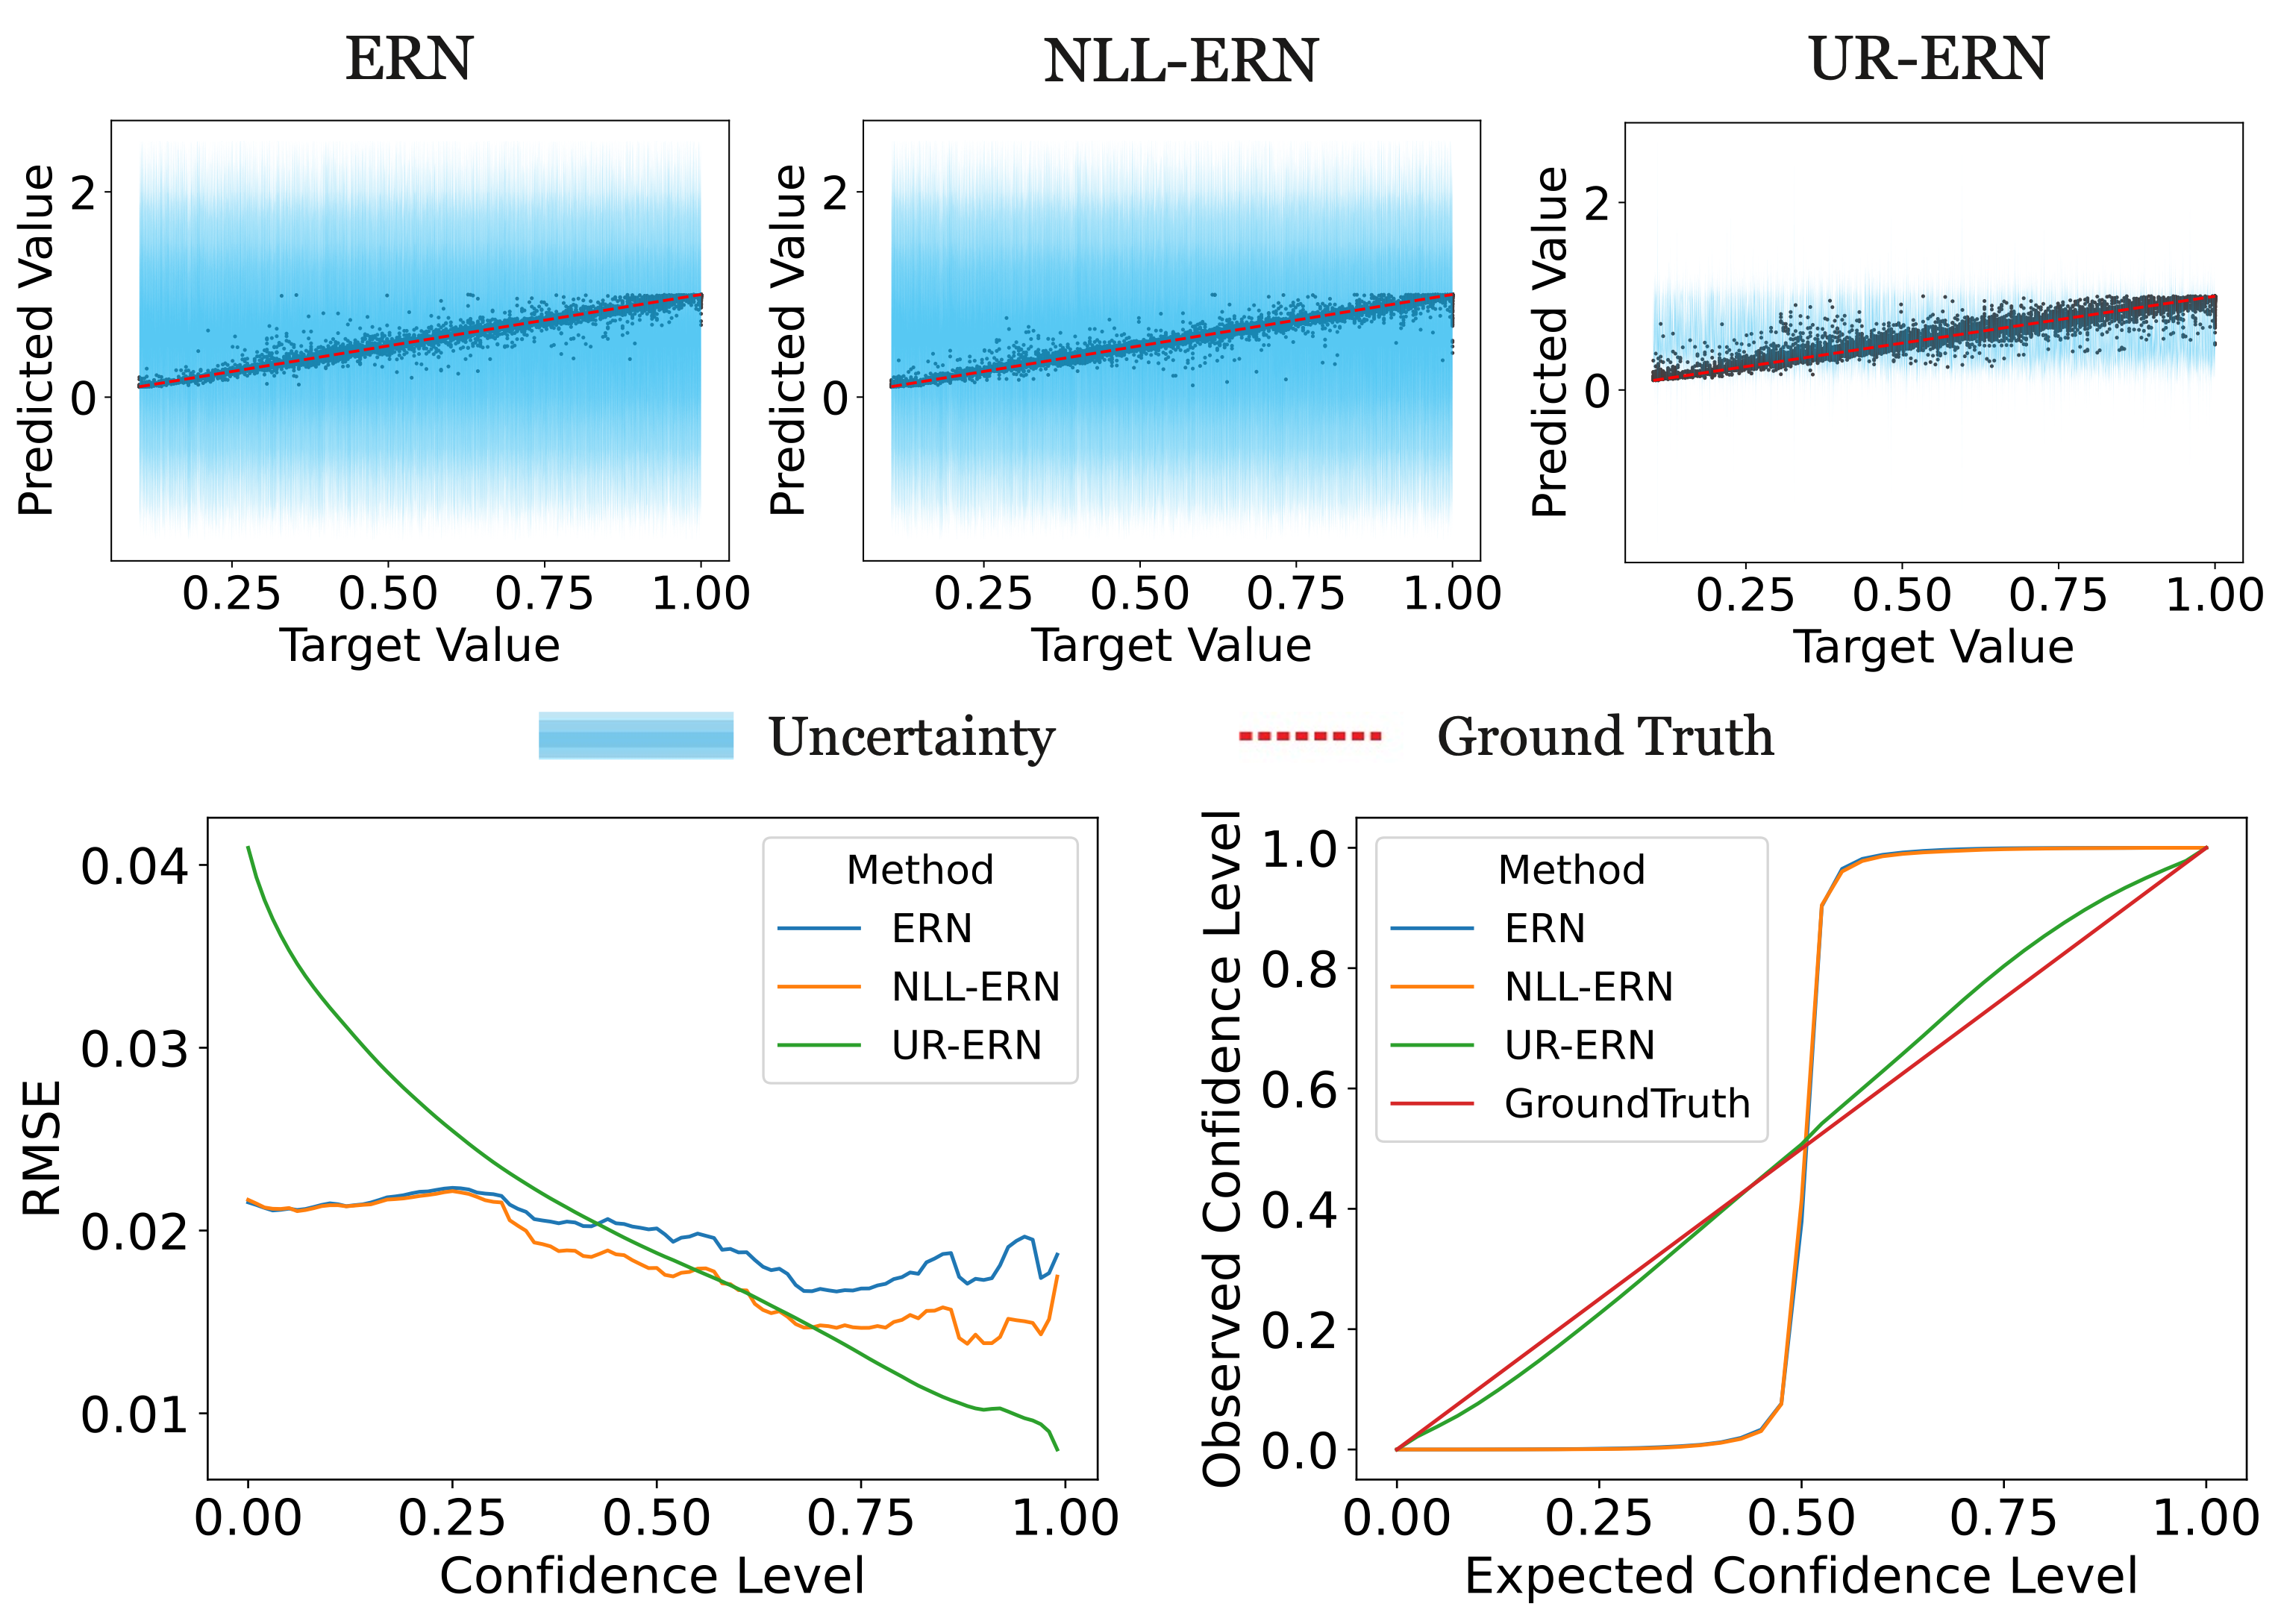
\includegraphics[width=0.9\columnwidth]{depth_HUA.png} % Reduce the figure size so that it is slightly narrower than the column. Don't use precise values for figure width.This setup will avoid overfull boxes.
% \caption{Uncertainty prediction of depth estimation within HUA.}
% \label{fig:depth_HUA}
% \end{figure}


Figure~\ref{fig:depth_HUA} presents a comparison of model performances as pixels possessing uncertainty beyond specific thresholds are excluded. The proposed \ours demonstrates robust behavior, characterized by a consistent reduction in error corresponding to increasing levels of confidence. In addition to the performance comparison, Figure~\ref{fig:depth_HUA} provides an assessment of the calibration of our uncertainty estimates. The calibration curves, computed following the methodology described in previous work~\cite{kuleshov2018accurate}, should ideally follow $y=x$ for accurate representation. The respective calibration errors for each model are also shown. 



\subsubsection{Monocular Depth Estimation outside HUA}
We also look at how the models perform outside the HUA. Figure~\ref{fig:depth_outside_HUA} visualizes the comparison of how the models can estimate uncertainty in depth estimation outside HUA. The proposed \ours has a lower Root Mean Square Error (RMSE) for most confidence levels than the competing models. And the calibration curve is closer to the ideal curve $y=x$ than any competing model, showing again the effectiveness of the proposed \ours.

For OOD experiments, the proposed \ours can distinguish OOD data better than the competing models. The above experiments reveal that the proposed regularization can not only be effective at guiding the model to get out of HUA, but it also performs well outside HUA. 

% \begin{figure}
% \centering
% 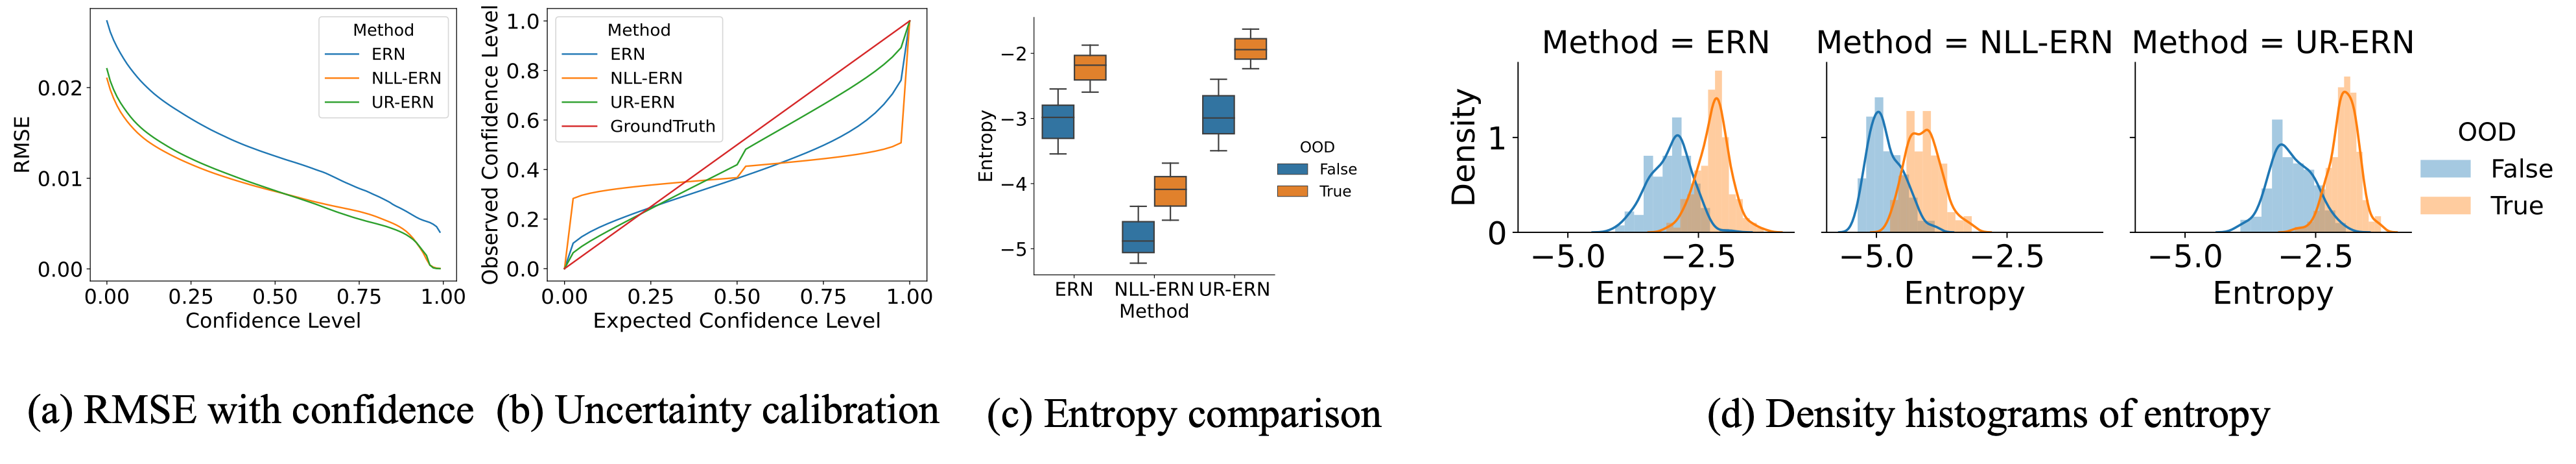
\includegraphics[width=0.9\columnwidth]{depth_outside_HUA.png} % Reduce the figure size so that it is slightly narrower than the column. Don't use precise values for figure width.This setup will avoid overfull boxes.
% \caption{Uncertainty prediction of depth estimation within HUA.}
% \label{fig:depth_outside_HUA}
% \end{figure}
% \begin{figure}
%   \centering
%   \subfloat[]{
%     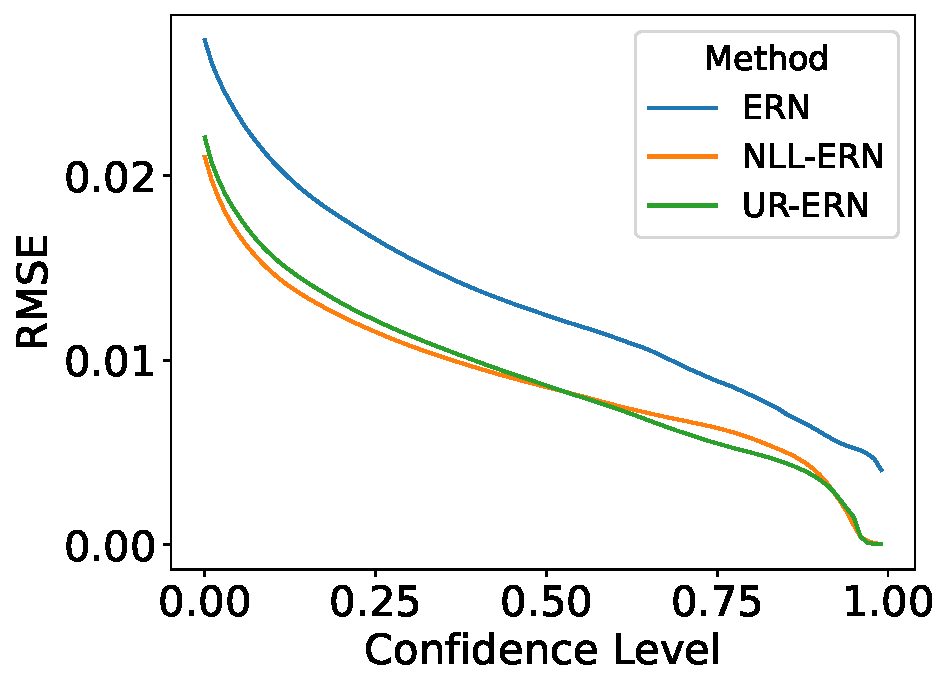
\includegraphics[width=0.45\linewidth]{depth_outside_HUA_1.pdf}
%   }
%   \subfloat[]{
%     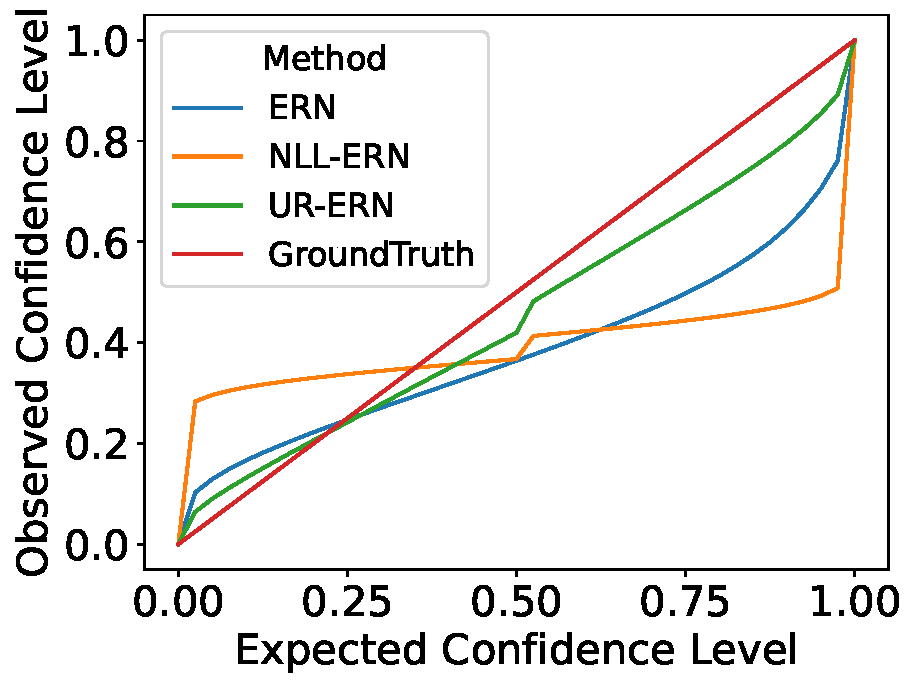
\includegraphics[width=0.45\linewidth]{depth_outside_HUA_2.pdf}
%   }\\
%   \subfloat[]{
%     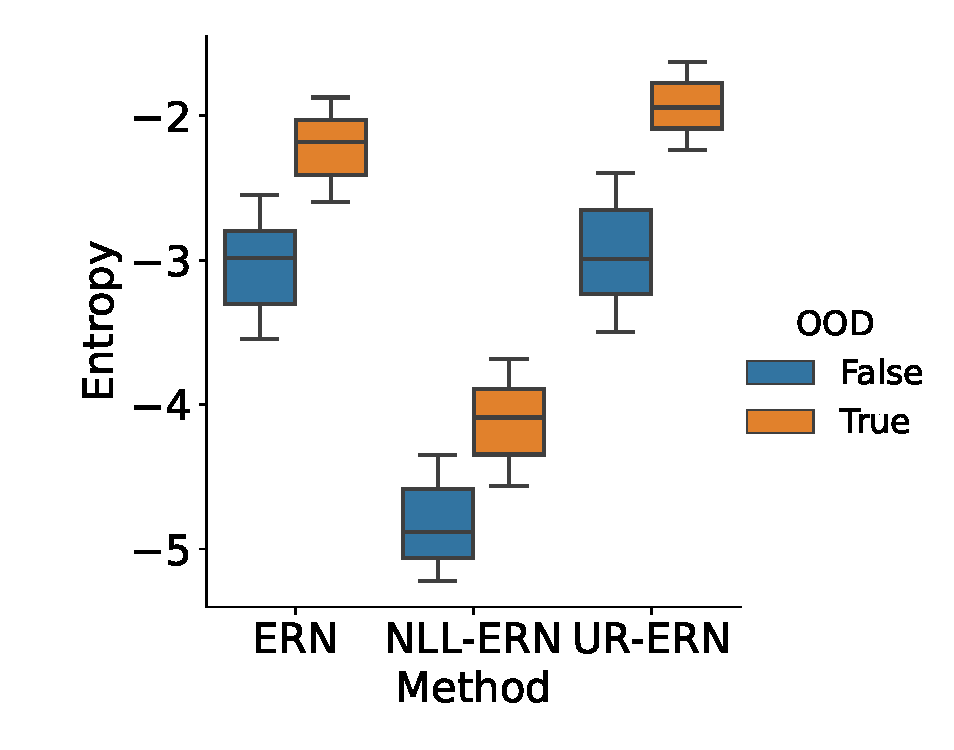
\includegraphics[width=0.5\linewidth]{depth_outside_HUA_3.pdf}
%   }\\
%   \subfloat[]{
%     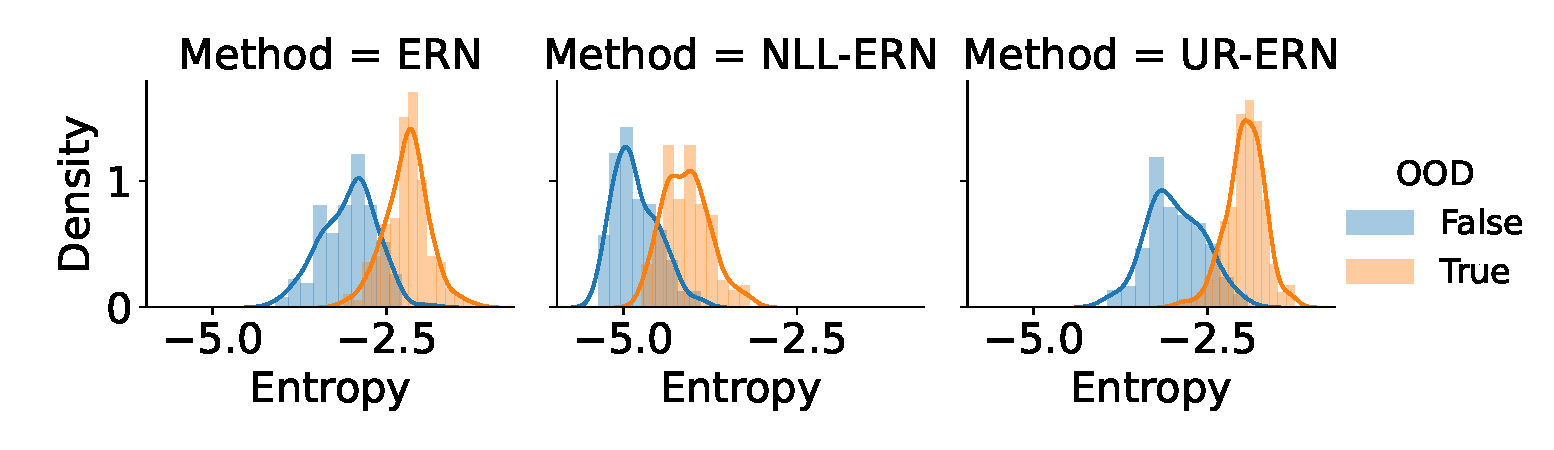
\includegraphics[width=0.9\linewidth]{depth_outside_HUA_4.pdf}
%   }
%   \caption{Uncertainty prediction of depth estimation outside HUA.}
%   \label{fig:depth_outside_HUA}
% \end{figure}

\subsection{Extension to Different ERN Variants}
Our theoretical findings reveal that the performance issues within HUA extend beyond ERN. Other evidential models, even those utilizing different prior distributions, similarly exhibit poor performance within this challenging region. 

Following the theoretical analysis in the previous section, we compare the performance of models in the context of Multivariate Deep Evidential Regression~\cite{meinert2021multivariate}. Following the experimental setup in~\cite{meinert2021multivariate}, we conduct the multivariate experiment and predict $(x, y) \in \mathbb{R}^2$ given $t \in \mathbb{R}$, where $x$ and $y$ being the features of the data sample given input $t$ with the following definition:
\begin{equation}
x=(1+\epsilon) \cos t, \quad 
y=(1+\epsilon) \sin t,
\end{equation}
and the distribution of $t$ is formulated as following:
\begin{equation}
t \sim \begin{cases}1-\frac{\zeta}{\pi} & \text { if } \zeta \in[0, \pi] \\ \frac{\zeta}{\pi}-1 & \text { if } \zeta \in(\pi, 2 \pi] \\ 0 & \text { else }\end{cases}
\end{equation}
where $\zeta \in[0,2 \pi]$ is uniformly distributed and $\epsilon \sim \mathcal{N}(0,0.1)$ is drawn from a normal distribution. Under this setting, the uncertainty is calculated as $\frac{\boldsymbol{L} \boldsymbol{L}^{\top}}{\nu-3}$. When $\nu\rightarrow3$, the corresponding uncertainty will be infinite across the dataset. Similar to previous experiments, we initialize the model within HUA by setting bias in the activation layer (See details in Appendix~\ref{appendix_2}).


% \begin{figure}
%     \centering
%     \begin{subfigure}{0.5\columnwidth}
%         \centering
%         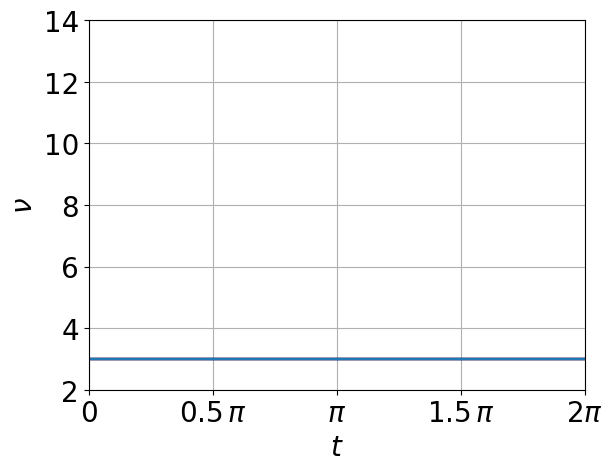
\includegraphics[width=0.95\linewidth]{nu_MERN.png}
%         \caption{Multivariate ERN}
%         %\label{fig:image_cutoff}
%     \end{subfigure}%
%         \begin{subfigure}{0.5\columnwidth}
%         \centering
%         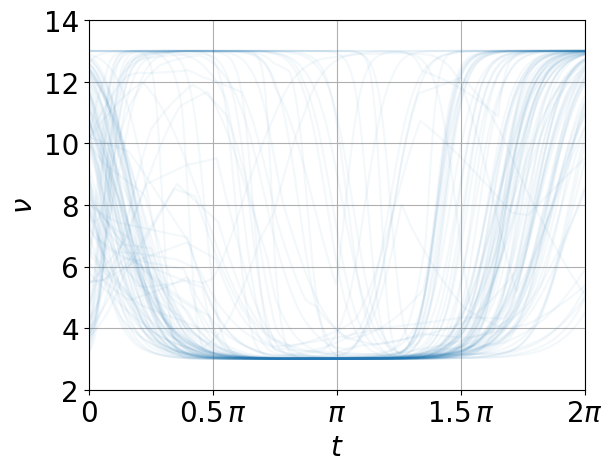
\includegraphics[width=0.95\linewidth]{nu_URERN.png}
%         \caption{\ours}
%         %\label{fig:image_calib}
%     \end{subfigure}
%     \caption{Prediction of parameter $\nu$ of Multivariate ERN and our proposed \ours. Low (high) values correspond to large (low) uncertainty prediction.}
%     \label{fig:multivariate}
% \end{figure}



Figure~\ref{fig:multivariate}(a) shows that the Multivariate ERN struggles to update the parameter $\nu$, resulting in unreasonably high uncertainty estimations (see Appendix~\ref{appendix_2} for additional experimental results). Consistent with previous sections, the proposed \ours in Figure~\ref{fig:multivariate}(b) does not encounter this issue, effectively learning from samples within HUA and providing reasonable uncertainty predictions. This validates our theoretical findings, demonstrating that evidential models, including but not limited to ERN, face challenges in the HUA when utilizing specific activation functions to ensure non-negative values. As a solution to this problem, our proposed uncertainty regularization term $\mathcal{L}^{\mathrm{U}}$ can be universally applied to these methods, enabling them to avoid the issue of zero gradients in the HUA.


\begin{figure}[h!]
    \centering
    \subfloat[Multivariate ERN]{
        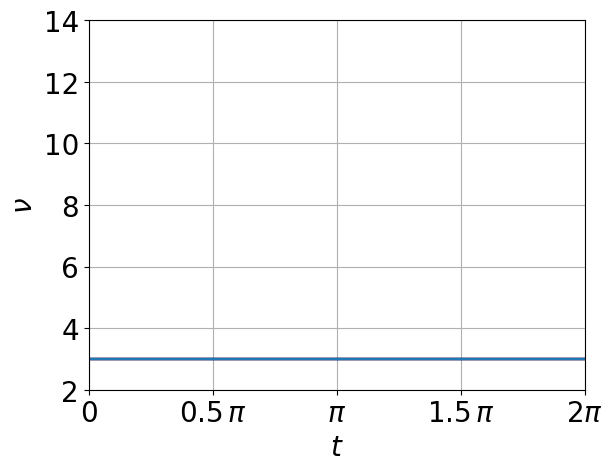
\includegraphics[width=0.45\linewidth]{nu_MERN.png}
        %\label{fig:image_cutoff}
    }
    \subfloat[\ours]{
        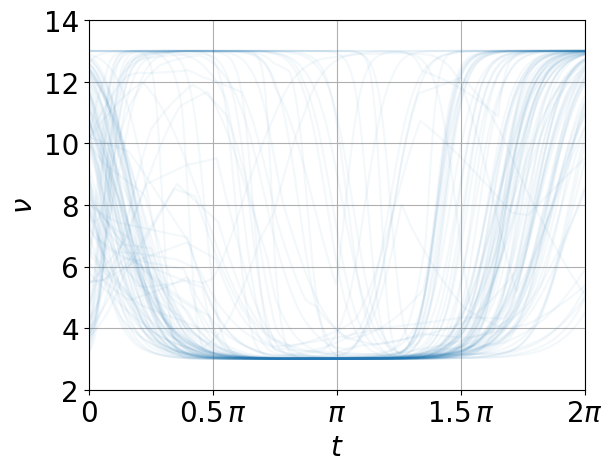
\includegraphics[width=0.45\linewidth]{nu_URERN.png}
        %\label{fig:image_calib}
    }
    \caption{Prediction of parameter $\nu$ in Multivariate ERN and our proposed \ours. Uncertainty ($\frac{\boldsymbol{L} \boldsymbol{L}^{\top}}{\nu-3}$) will be infinite if $\nu$ is close to 3, indicating the evidential model fails to properly estimate the uncertainty of predictions.}
    \label{fig:multivariate}
\end{figure}

% \begin{figure}
%     \centering
%     \subfloat[Multivariate ERN]{
%         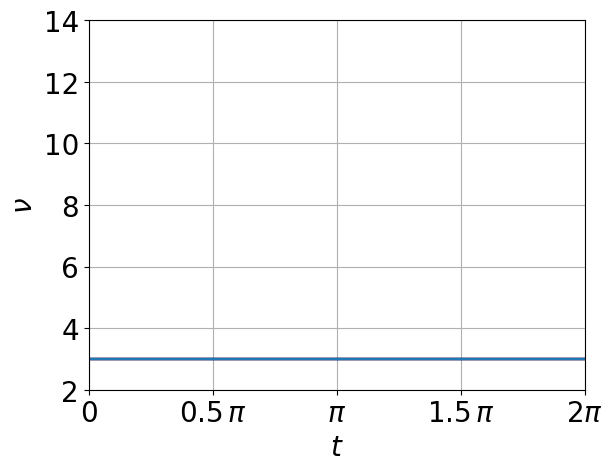
\includegraphics[width=0.45\linewidth]{nu_MERN.png}
%         %\label{fig:image_cutoff}
%     }
%     \subfloat[\ours]{
%         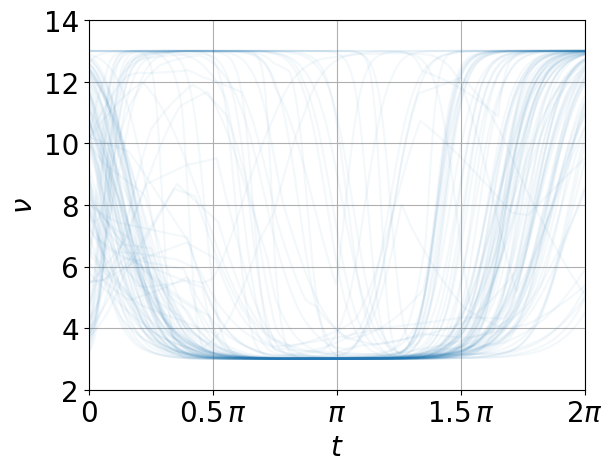
\includegraphics[width=0.45\linewidth]{nu_URERN.png}
%         %\label{fig:image_calib}
%     }
%     \caption{Prediction of parameter $\nu$ of Multivariate ERN and our proposed \ours. Low (high) values correspond to large (low) uncertainty prediction.}
%     \label{fig:multivariate}
% \end{figure}